\documentclass[11pt,a4paper]{article}
\usepackage{fullpage}
\usepackage{amsmath}
\usepackage{amssymb}
\usepackage{amsfonts}
\usepackage{mathtools}
\usepackage{titlesec}
\usepackage{graphicx}
\usepackage{float}
\usepackage{wrapfig}
\usepackage{multicol}
\usepackage{caption}
\usepackage{hyperref}
\usepackage{apacite}
\usepackage{multirow}

\titleformat*{\section}{\large\bfseries}

\begin{document}
	
	\title{\textbf{Rendering Lab Report}}
	\author{\textbf{Adil Rabbani} \\ \textbf{Advisor: Prof. 
			Dr.-Ing. Matthias Teschner}}
	\maketitle
	
	\section{Introduction}
	The aim of this lab is to build a simple ray tracer capable of rendering images using some of the concepts we learned in our computer graphics course. I would like to thank \textbf{Prof. Dr.-Ing. Matthias Teschner} for advising me throughout this lab. I would also like to mention some important resources I used to build the ray tracer including, \textbf{Peter Shirley's Ray tracing in One Weekend} \cite{Shirley2020RTW1}, \textbf{Kevin Suffern's Ray tracing from the Ground Up} \cite{suffern2016ray} and \textbf{Scratch a pixel} \cite{scratchapixel} which is a blog comprising of explanations of different concepts about ray tracing. Other than these resources, I have used a couple of other resources including \textbf{Wikipedia} for which I have given references where ever necessary.
	
	\section{Why Ray tracing?}
	One of the biggest motivation in the field of Computer Graphics is to create virtual environments that look as close to how they look in real life. \textbf{Ray tracing} is capable of producing highly realistic images that have various applications including but not limited to movies, simulation as well as video games (recently). Ray tracing, unlike \textbf{rasterization} is capable of simulating light transport because of all the interactions between lights and objects. Disney's \textbf{Hyperion Renderer} for example is a Path tracer (an efficient ray tracing technique) which helps produce their animated movies.
	\begin{figure}[H]
		\centering
		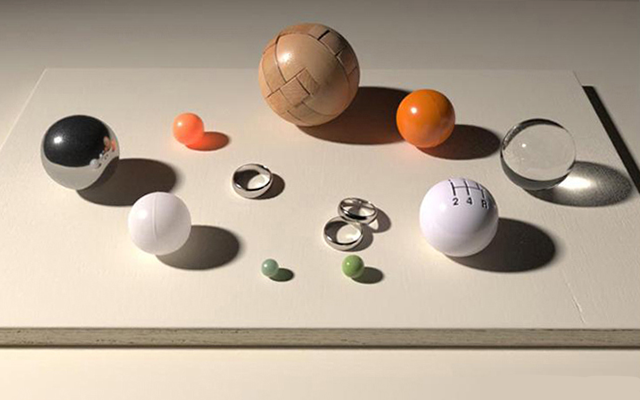
\includegraphics[width=0.7\textwidth]{hyperion_renderer.png}
		\caption{\centering An image rendered by Disney's Hyperion Renderer \protect\cite{burley2018design}.}
	\end{figure}
	\noindent
	As you can observe in the image above, it is almost impossible to figure out if this is an actual photograph of real world objects or rendered by a computer. You can also notice how different objects are able to simulate different material properties similar to how they look in real life. Nowadays, the use of ray tracing is also becoming main stream in interactive applications such as video games because of the development of high performance GPUs. \textbf{NVIDIA Marbles} for example, is a fully playable physics based game which also makes use of recently introduced Nvidia's RTX (real-time ray tracing) technology. 
	\begin{figure}[H]
		\centering
		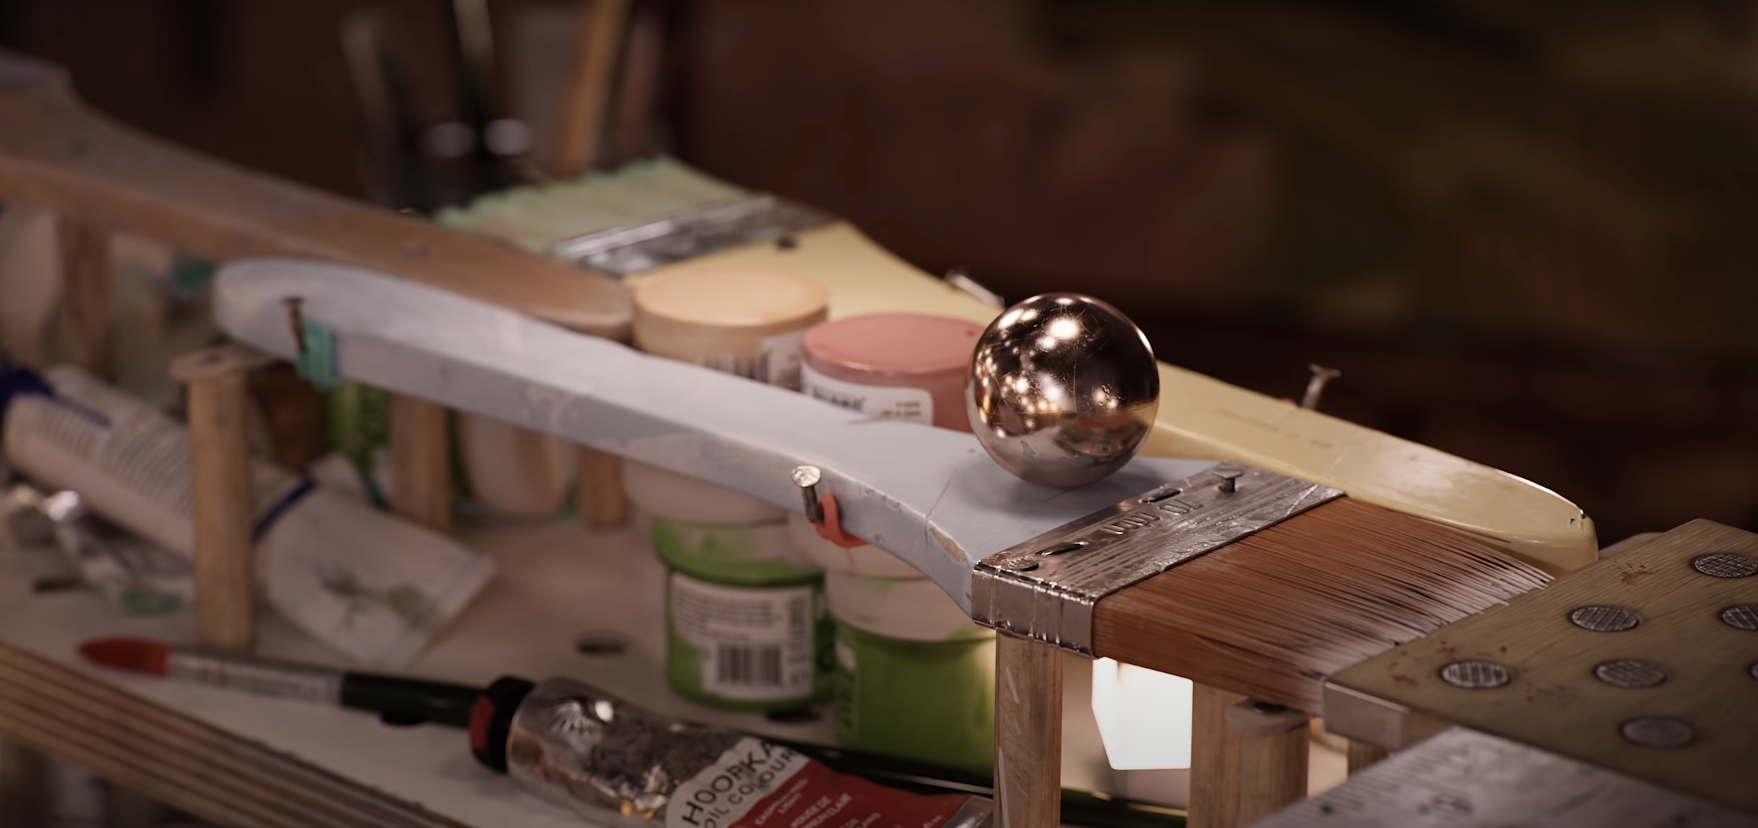
\includegraphics[width=0.7\textwidth]{nvidia_marbles.png}
		\caption{\centering A snapshot of NVIDIA Marbles at Night Demo. \protect\cite{nvidiamarbles}.}
	\end{figure}
	\noindent
	So these examples clearly demonstrate that ray tracing can be used in a variety of applications while also giving more realistic results. While it is still quite expensive as compared to rasterization it is becoming more and more mainstream as the computing potential in GPUs and CPUs improve from time.
	
	\section{How ray tracing works?}
	\begin{figure}[H]
		\centering
		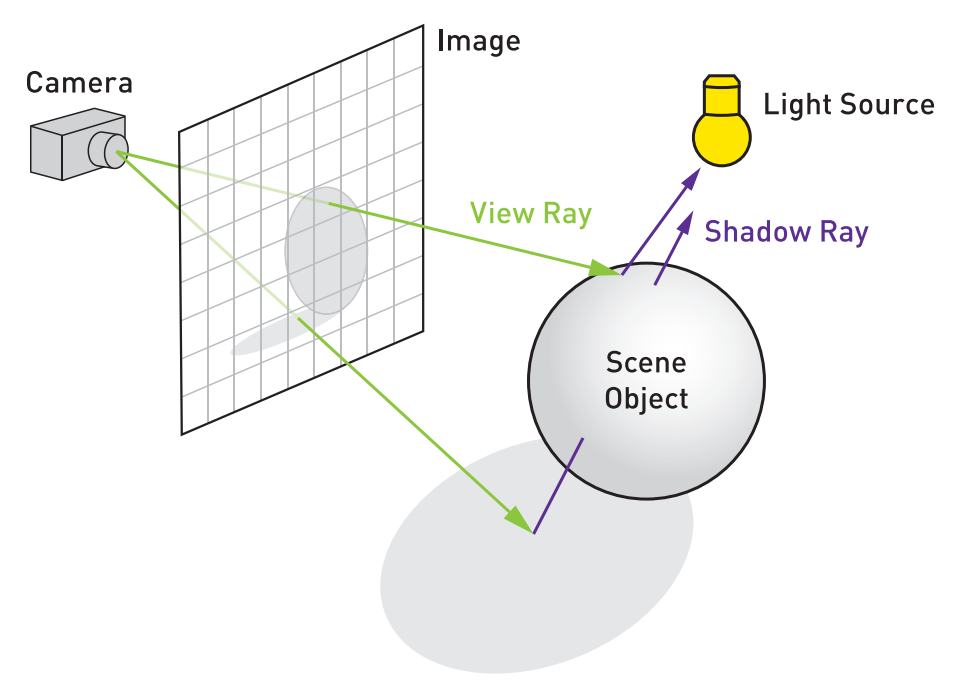
\includegraphics[width=0.6\textwidth]{raytracing_gems.png}
		\caption{\centering An image showing how a ray is casted from the camera and how objects are illuminated and shadows are computed in ray tracing \protect\cite{haines2019ray}.}
	\end{figure}
	Ray tracing makes use of \textbf{ray casting} to compute the closest hit point with an object. This is done by a camera that shoots multiple rays from each pixel of the image. These rays then intersect with an object in the scene which is evaluated by a ray-object intersection method. Each object in our scene also have different material properties that bounce off light differently. Shadows are computed by sending another ray from the hit point towards the light source and if this ray hits another object on its way towards the light source, then that hit point is in shadow. This process can be done recursively to get more realistic results keeping a recursion cut off limit. The aim of ray tracing is to compute the overall light transport in a scene while illuminating surfaces according to their material properties.

	\section{Implementation Details}
	The accompanied ray tracer uses C++ programming language to implement it. I worked on this ray tracer using many resources but the initial structure follows the one explained in \textbf{Peter Shirley's Ray tracing in One Weekend} \cite{Shirley2020RTW1} therefore, some parts of the code are quite similar to that book. The code was implemented and tested on a machine with Ubuntu 20.04.2 LTS. Here, I will mention briefly the structure of the ray tracer.
	\subsection{External Libraries}
	The ray tracer uses two external libraries. Both of these libraries are single file header only, so nothing needs to be installed in order to make the code run.
	\begin{enumerate}
		\item \textbf{pnm:} This is a ppm image read/write library for C++. This is to facilitate in loading different kinds of textures as some ppm files usually have a binary encoding.
		\item \textbf{tinyobjloader:} This is a light weight .obj format parser for C++. This is to facilitate in loading different .obj format meshes.
	\end{enumerate}
	\subsection{Code Structure}
	\begin{enumerate}
		\item \textbf{camera.h, vec3.h, sphere.h, color.h, constants.h, hittable.h, ray.h} \\
		These header files are quite similar to how they were implemented in Ray tracing in One Weekend. \textbf{cam.h} implements a perspective camera. \textbf{vec3.h} implements the vector class along with different vector helper functions. \textbf{color.h} has a function that writes the color of the pixel to an image file. \textbf{constants.h} have some global helper functions and constants.  \textbf{hittable.h} contains a struct that saves the hit point properties when a ray is hit with an object. \textbf{sphere.h} is the sphere class with its definitions as well as its intersect method. The intersect method is the same as the one being used in the book but it also adds functionality for textures in it. \textbf{ray.h} is the ray class.
		
		\item \textbf{triangle.h, aabb.h, light.h, mesh.h, texture.h, scene.h} \\
		These header files are a mix of different resources I went through in order to implement them. This includes going through different books as well as articles. \textbf{triangle.h} is the triangle class with its definitions as well as the intersect method. The intersect method follows the one by \cite{raytriangle} which is the same algorithm I've explained in the report. \textbf{aabb.h} is axis aligned bounding boxes implementation and follows the one explained at \cite{scratchapixel}. \textbf{light.h} has two different light classes. The random sampling of positions in area lights follows an implementation discussed at \cite{stackoverflow}. \textbf{mesh.h} uses tinyobjloader to load a mesh. \textbf{texture.h} has a texture class that uses pnm to load a texture. \textbf{scene.h} is the biggest class in the ray tracer and implements phong illumination and implements how a hit point is shaded according to the type of light used. This also implements antialiasing as explained in Ray tracing in One Weekend \cite{Shirley2020RTW1}.
		
	\end{enumerate}
	
	\section{Using PPM (Portable Pixmap) format to generate images}
	
	PPM (Portable Pixmap) image format is used to generate images. One reason for using this format is that it is easier to generate images in this format as compared to other formats. It is based on RGB color space, red(R), green(G) and blue(B). The color component can be specified by a value between 0 and a maximum value of 255. A typical PPM image file looks like this:\\
	\\
	\texttt{P3} \\
	\texttt{\# P3 means colors are in ASCII, then 3 columns and 3 rows,} \\
	\texttt{\# then 255 for max color, then RGB triplets}\\
	\texttt{3 3}\\
	\texttt{255}
	\begin{tabbing}
		\texttt{255 0 0 \hspace*{1.55cm} 0 255 0 \hspace*{1.98cm} 0 0 0}\\
		\texttt{0 0 255 \hspace*{1.55cm} 255 255 0 \hspace*{1.55cm} 255 0 255}\\
		\texttt{255 255 255 \hspace*{0.7cm} 0 255 255 \hspace*{1.53cm} 255 100 0}
	\end{tabbing}
	which generates an image:
	 \begin{figure}[H]
		\centering
		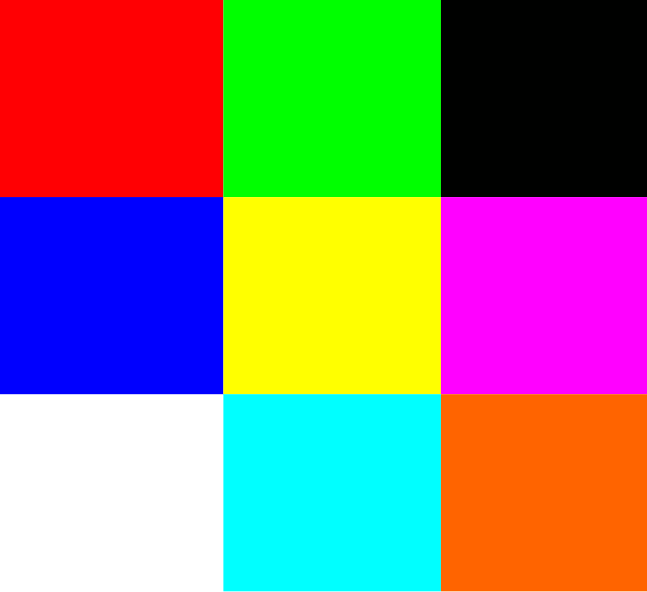
\includegraphics[width=3cm]{ppm_example.png}
		\caption{\centering A ppm image with the values as mentioned above. This example is magnified as these are individual pixel colors and might show up small on an actual image \protect\cite{ppmformat}.}
	 \end{figure}

	\section{Sending rays into the scene}
	A ray can be defined as a function $\boldsymbol{p}(t) = \boldsymbol{o} + t\boldsymbol{d}$ where $\boldsymbol{p}$ is a position along a line in 3D. $\boldsymbol{o}$ is the origin (the starting point of the ray) while $\boldsymbol{d}$ is the ray direction. $t$ is how far we want the ray to travel in the direction $\boldsymbol{d}$.\\
	\begin{figure}[H]
		\centering
		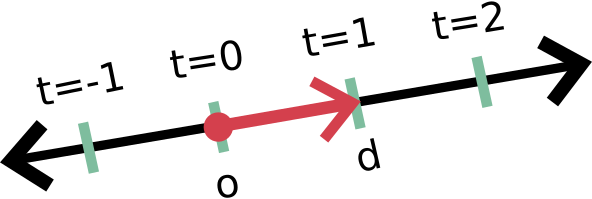
\includegraphics[width=8cm]{ray1.png}
		\caption{\centering A ray with origin $\boldsymbol{o}$ at $t=0$ going towards $t=1$ with a direction $\boldsymbol{d}$ \protect\cite{Shirley2020RTW1}.}
	\end{figure}
	\noindent
	There are 3 important steps for a ray tracer:
	\begin{enumerate}
		\item Calculate the primary ray from the eye (camera) to the pixel.
		\item Determine the ray's closest intersection with an object.
		\item Compute a color for that intersection point.
	\end{enumerate}

	\noindent
	For setting up the camera we'll set the $y-axis$ to go up, the $x-axis$ to the right and the negative $z-axis$ into the screen as shown in the figure below:
	\begin{figure}[H]
		\centering
		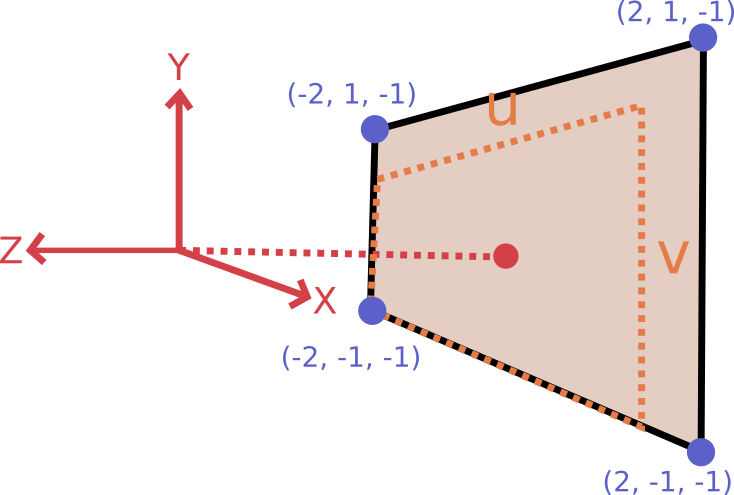
\includegraphics[width=8cm]{camera.png}
		\caption{\centering A camera(eye) setup \protect\cite{Shirley2020RTW1}.}
	\end{figure}

	\section{Adding a triangle to the scene (ray-triangle intersection)}
	\subsection{Introduction}
	In computer graphics, most 3D models are triangulated (you can make up any geometry combining a bunch of triangles into a triangular mesh) so starting with the most important shape is a good idea.\\
	
	There are some properties related to vectors that are important here:
	\begin{enumerate}
		\item Subtracting a point $a$ from a point $b$ in space would give you a vector $\boldsymbol{a}$ along the direction of $\boldsymbol{b}$.
		\item A cross product between two vectors, $\boldsymbol{a} \times \boldsymbol{b}$  gives a vector that is perpendicular to both of them. This is important in our case because this allows us to get the normal, $\boldsymbol{n}$ of the plane our triangle lies in.
		\begin{figure}[H]
			\centering
			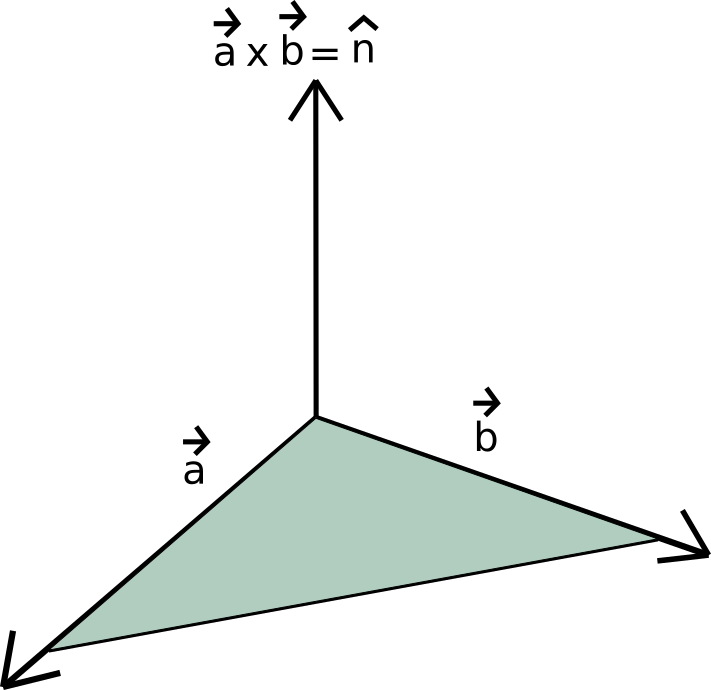
\includegraphics[width=6cm]{axb_normal.png}
			\caption{\centering Vector $\boldsymbol{a}$ and $\boldsymbol{b}$ and the normal $\boldsymbol{\hat{n}}$.}
		\end{figure}
		\item A dot product between two vectors, $\boldsymbol{a}.\boldsymbol{b}$, if $0$, means that the vectors are orthogonal to each other.
	\end{enumerate}	

	\subsection{Barycentric Coordinates}
	We all know defining a triangle is easy. We can have three points in space and can define a triangle. But we need to somehow figure out the position of a given point $\boldsymbol{p}$ in space given three points of a triangle.
	
	\begin{figure}[H]
		\centering
		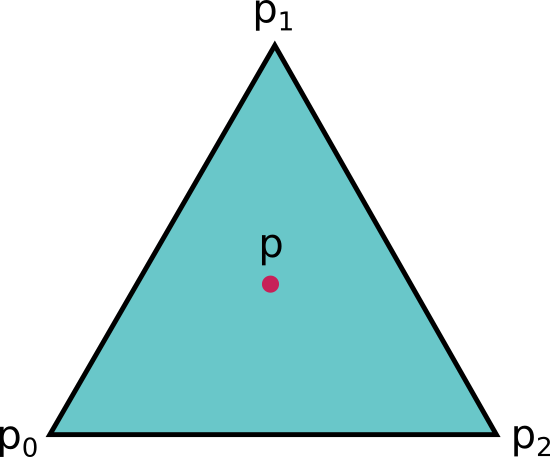
\includegraphics[width=5cm]{triangle.png}
		\caption{\centering Three points, $\boldsymbol{p}_{0}$, $\boldsymbol{p}_{1}$ and $\boldsymbol{p}_{2}$ make up a triangle. A point $\boldsymbol{p}$ lies on that triangle \protect\cite{trianglemeshes}.}
	\end{figure}
	
	\noindent
	Because triangles are planar surface and the points that make up the triangle uniquely define that plane. Any point $\boldsymbol{p}$ on that plane, can be represented as a linear combination of the points that make up the triangle. So in our example above, our point $\boldsymbol{p}$ can be represented as a linear combination of the points, $\boldsymbol{p}_{0}$, $\boldsymbol{p}_{1}$ and $\boldsymbol{p}_{2}$:
	\begin{equation}
	\boldsymbol{p} = \alpha \boldsymbol{p}_{0} + \beta \boldsymbol{p}_{1} + \gamma \boldsymbol{p}_{2}
	\end{equation}
	
	\noindent
	These $\alpha$, $\beta$ and $\gamma$ are called the Barycentric Coordinates of this point $\boldsymbol{p}$ on this triangle. These are the weights (in simpler terms) that we could use to determine the position of point $\boldsymbol{p}$ using a linear combination of the vertices $\boldsymbol{p}_{0}$, $\boldsymbol{p}_{1}$ and $\boldsymbol{p}_{2}$. These barycentric coordinates also have a very important property which is:
	\begin{equation}
	\alpha + \beta + \gamma = 1
	\end{equation}
	
	\noindent
	Note, that if we know any of the two barycentric coordinates, $\alpha$ and $\beta$, we can get the third one as $\gamma = 1 - \alpha - \beta$ as they must add upto $1$. One important thing to mention is that we can represent any point on the infinite plane our triangle lies in, using these coordinates. This includes a point $\boldsymbol{p}$ which is outside our triangle. But if our point $\boldsymbol{p}$ is on the triangle, we have an additional property that our barycentric coordinates would always be positive and smaller than $1$:
	\begin{equation}
	0 \le \alpha \le 1 \;\;\;\;\; 0 \le \beta \le 1 \;\;\;\;\; 0 \le \gamma \le 1
	\end{equation}
	
	\noindent
	One advantage of using barycentric coordinates is that they could be used to define attributes (color or texture) on a triangle because we are essentially linearly interpolating between the three vertices of a triangle.
	
	\subsection{Möller-Trumbore Algorithm}
	The \textbf{Möller-Trumbore Algorithm} is a fast ray-triangle intersection algorithm which was introduced by \textbf{Tomas Möller} and \textbf{Ben Trumbore} in 1997 in their paper titled "Fast, Minimum Storage Ray/Triangle Intersection" \cite{moller1997fast}.\\~\\
	\noindent
	A point, $\boldsymbol{t}(\alpha, \beta)$, on a triangle can be represented as:
	\begin{equation}
	\boldsymbol{t}(\alpha, \beta) = (1 - \alpha - \beta)\boldsymbol{p}_{0} + \alpha\boldsymbol{p}_{1} + \beta\boldsymbol{p}_{2}
	\end{equation}
	\noindent
	Here, $(\alpha, \beta)$ are the barycentric coordinates of a triangle which hold all the properties we mentioned above. The intersection between ray, $\boldsymbol{p}(t)$, and the triangle, $\boldsymbol{t}(\alpha, \beta)$, is equivalent so:
	\begin{equation}
		\boldsymbol{o} + t\boldsymbol{d} = (1 - \alpha - \beta)\boldsymbol{p}_{0} + \alpha\boldsymbol{p}_{1} + \beta\boldsymbol{p}_{2}
	\end{equation}
	Expanding this equation, we get:
	\begin{equation}
		\boldsymbol{o} + t\boldsymbol{d} = \boldsymbol{p}_{0} - \alpha\boldsymbol{p}_{0} - \beta\boldsymbol{p}_{0} + \alpha\boldsymbol{p}_{1} + \beta\boldsymbol{p}_{2}
	\end{equation}
	And rearranging we get:
	\begin{equation}
		\boldsymbol{o} - \boldsymbol{p}_{0} = -t\boldsymbol{d} + \alpha(\boldsymbol{p}_{1} - \boldsymbol{p}_{0}) + \beta(\boldsymbol{p}_{2} - \boldsymbol{p}_{0})
	\end{equation}
	\noindent
	We have three unknowns here $t, \alpha, \beta$ with four known terms $\boldsymbol{o}, (\boldsymbol{p}_{1} - \boldsymbol{p}_{0}), (\boldsymbol{p}_{2} - \boldsymbol{p}_{0})$ and $\boldsymbol{d}$. We can again rearrange these terms into the form:
		\[
		\left[
		\begin{array}{ccc}
		-\boldsymbol{d} & (\boldsymbol{p}_{1} - \boldsymbol{p}_{0}) & (\boldsymbol{p}_{2} - \boldsymbol{p}_{0}) 
		\end{array}
		\right]
		\begin{bmatrix}
		t \\
		\alpha \\
		\beta 
		\end{bmatrix} = \boldsymbol{o} - \boldsymbol{p}_{0}
		\]
	This means, that solving the above linear system of equations, we can get our three unknowns $(t, \alpha, \beta)$. You can notice, that the authors of the paper are representing the coordinates of the point $\boldsymbol{t}$ in terms of $\alpha$ and $\beta$ (the barycentric coordinates) of the triangle and not in terms of $x$, $y$ and $z$. We know that $\alpha$ and $\beta$ both can't be lower than $0$ and $\alpha + \beta \le 1$ so our triangle is in fact a unit triangle.\\~\\
	\noindent
	We denote $\boldsymbol{e}_{1} = (\boldsymbol{p}_{1} - \boldsymbol{p}_{0})$, $\boldsymbol{e}_{2} = (\boldsymbol{p}_{2} - \boldsymbol{p}_{0})$ and $\boldsymbol{c} = \boldsymbol{o} - \boldsymbol{p}_{0}$, then by \textbf{Cramer's Rule} \cite{cramersrule} we can solve the above system of equations as:
	\[
	\begin{bmatrix}
	t \\
	\alpha \\
	\beta 
	\end{bmatrix} = \left[
	\begin{array}{ccc}
	\frac{1}{|-\boldsymbol{d},\;\;\boldsymbol{e}_{1},\;\;\boldsymbol{e}_{2}|}
	\end{array}
	\right]
	\
	\begin{bmatrix}
	|\;\;\boldsymbol{c},\;\;\boldsymbol{e}_{1},\;\;\boldsymbol{e}_{2}\;\;| \\
	|-\boldsymbol{d},\;\;\boldsymbol{c},\;\;\boldsymbol{e}_{2}| \\
	|-\boldsymbol{d},\;\;\boldsymbol{e}_{1},\;\;\boldsymbol{c}|
	\end{bmatrix}
	\]
	where $|-\boldsymbol{d},\;\;\boldsymbol{c},\;\;\boldsymbol{e}_{2}|$ is the determinant of the matrix having columns, $-\boldsymbol{d}$, $\boldsymbol{c}$ and $\boldsymbol{e}_{2}$. Finally, since we are dealing with vectors, we can use the property: 
	\begin{equation}
	|\boldsymbol{u},\;\boldsymbol{v},\;\boldsymbol{w}| = -(\boldsymbol{u}\;\times\;\boldsymbol{w})\;\cdot\;\boldsymbol{v} = -(\boldsymbol{w}\;\times\;\boldsymbol{v})\;\cdot\;\boldsymbol{u}
	\end{equation}
	and write our solution as:
	\[
	\begin{bmatrix}
	t \\
	\alpha \\
	\beta
	\end{bmatrix} = \left[
	\begin{array}{ccc}
	\frac{1}{(\boldsymbol{d}\;\times\;\boldsymbol{e}_{2})\;\cdot\;\boldsymbol{e}_{1}}
	\end{array}
	\right]
	\
	\begin{bmatrix}
	(\boldsymbol{c}\;\times\;\boldsymbol{e}_{1})\;\cdot\;\boldsymbol{e}_{2} \\
	(\boldsymbol{d}\;\times\;\boldsymbol{e}_{2})\;\cdot\;\boldsymbol{c} \\
	(\boldsymbol{c}\;\times\;\boldsymbol{e}_{1})\;\cdot\;\boldsymbol{d}
	\end{bmatrix}
	\]
	or in a more concise way:
	\[
	\begin{bmatrix}
	t \\
	\alpha \\
	\beta 
	\end{bmatrix} = \left[
	\begin{array}{ccc}
	\frac{1}{\boldsymbol{p}\;\cdot\;\boldsymbol{e}_{1}}
	\end{array}
	\right]
	\
	\begin{bmatrix}
	\boldsymbol{q}\;\cdot\;\boldsymbol{e}_{2} \\
	\boldsymbol{p}\;\cdot\;\boldsymbol{c} \\
	\boldsymbol{q}\;\cdot\;\boldsymbol{d}
	\end{bmatrix}
	\]
	where $\boldsymbol{p}=(\boldsymbol{d}\;\times\;\boldsymbol{e}_{2})$ and $\boldsymbol{q}=(\boldsymbol{c}\;\times\;\boldsymbol{e}_{1})$.\\~\\
	We compute $t, \alpha$ and $\beta$ and return $-1\;(no\;intersection)$ if 
	\begin{equation}
		\alpha<0\;or\;\alpha>1\;or\;\beta<0\;or\;(\alpha\;+\;\beta)>1
	\end{equation}
	otherwise, there's an intersection and we return $t$, $\alpha$ and $\beta$.
	\begin{figure}[htp]
		\centering
		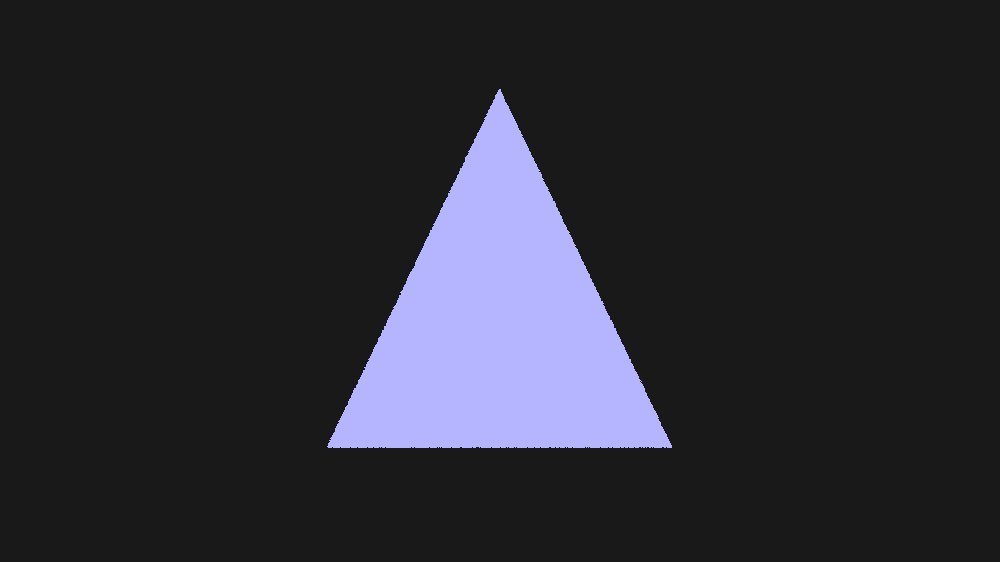
\includegraphics[width=.45\textwidth]{ray_triangle.png}\quad
		\caption{A triangle using normal as color value.}
	\end{figure}
	\section{Adding a sphere to the scene (ray-sphere intersection)}
	Let's start with circle first in order to get some intuition. The equation of a circle centered at origin of radius $r$ is $x^2+y^2=r^2$. If a given point $(x, y)$ is inside the circle, then $x^2+y^2<r^2$ and if it is outside the circle, then $x^2+y^2>r^2$. Considering the center is at $(c_{x}, c_{y})$, our equation becomes:
	\begin{equation}
	(x-c_{x})^2+(y-c_{y})^2=r^2
	\end{equation}
	An example would make it more clear. Consider a circle with its origin at $(4, 4)$ and radius $2$ along with three points, $\boldsymbol{p}_{0}(6, 4)$, $\boldsymbol{p}_{1}(5, 3)$ and $\boldsymbol{p}_{2}(6, 1)$. $\boldsymbol{p}_{0}$ is on the circle, $\boldsymbol{p}_{1}$ is inside while $\boldsymbol{p}_{2}$ is outside and we can verify this with our equation.
	\begin{figure}[H]
		\centering
		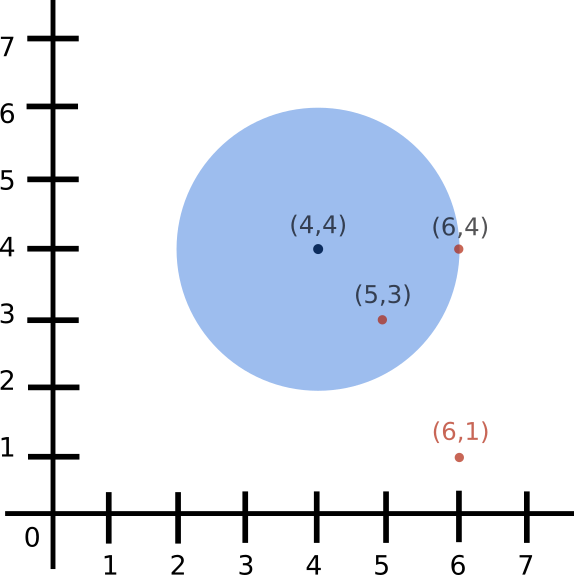
\includegraphics[width=6cm]{circle.png}
		\caption{\centering A circle with its origin at $(4, 4)$ along with 3 other points.}
	\end{figure}
	\noindent
	\begin{equation}
		(6-4)^2+(4-4)^2=(2)^2
	\end{equation}
	\begin{equation}
		(5-4)^2+(3-4)^2<(2)^2
	\end{equation}
	\begin{equation}
		(6-4)^2+(1-4)^2>(2)^2
	\end{equation}
	But since we want to render a sphere and not a circle we'll be using it's equation which is the same as circle's equation but with added dimension $z$. So our equation for sphere with its center at $(c_{x}, c_{y}, c_{z})$ is:
	\begin{equation}
	(x-c_{x})^2+(y-c_{y})^2+(z-c_{z})^2=r^2
	\end{equation}
	And the same rules for points being on, inside or outside the circle applies for sphere too. Since we are dealing with vectors, we need to change equation $(14)$ in vector form. Remember that a vector from a point $\boldsymbol{a}$ to point $\boldsymbol{b}$ is given by $\boldsymbol{b}-\boldsymbol{a}$, a vector from our center $\boldsymbol{c}$ to point $\boldsymbol{p}$ can similarly be given by $(\boldsymbol{p}-\boldsymbol{c})$ and equation $(14)$ becomes:
	\begin{equation}
	(\boldsymbol{p}-\boldsymbol{c})\cdot(\boldsymbol{p}-\boldsymbol{c})=r^2
	\end{equation}
	Adding our ray equation, to equation $(15)$ for all points $t$ that satisfies the equation we get:
	\begin{equation}
	(\boldsymbol{o} + t\boldsymbol{d}-\boldsymbol{c})\cdot(\boldsymbol{o} + t\boldsymbol{d}-\boldsymbol{c})=r^2
	\end{equation}
	Expanding equation $(16)$ and moving all terms to the left side we get:
	\begin{equation}
	t^2\boldsymbol{d}^2 + 2t\boldsymbol{d}\cdot(\boldsymbol{o} - \boldsymbol{c})+(\boldsymbol{o}-\boldsymbol{c})\cdot(\boldsymbol{o}-\boldsymbol{c})-r^2=0
	\end{equation}
	If you observe closely, equation $(17)$ is a quadratic equation with an unknown $t$. We can get the discriminant using the formula we all have learned in our high school:
	\begin{equation}
		b^2-4a \cdot c
	\end{equation}
	Our discriminant is zero when we have one real solution \textbf{(ray intersects the boundary of the sphere)}, it is positive when we have two real solutions \textbf{(ray intersects two points, the one where it enters and the other where it leaves)} and it is negative when we have no real solutions \textbf{(the ray did not intersect)}.

\begin{figure}[htp]
	\centering
	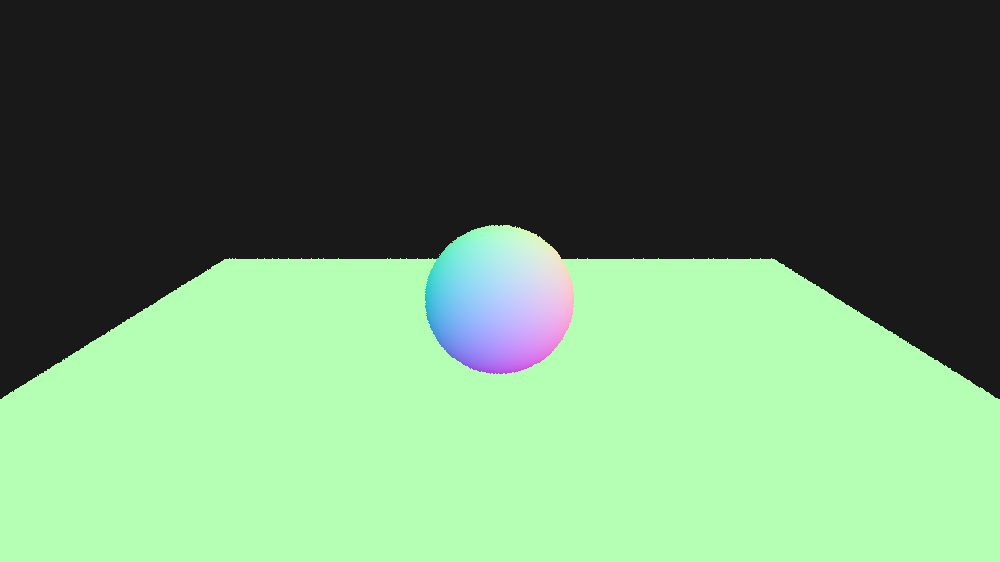
\includegraphics[width=.45\textwidth]{ray_sphere_triangle.png}\quad
	\caption{A sphere on a plane made up of two triangles using normal as color value.}
\end{figure}

	\section{Adding a triangular mesh to the scene}

\begingroup
\setlength{\intextsep}{0pt}
\setlength{\columnsep}{15pt}

\begin{wrapfigure}{r}{0.35\textwidth}
	\centering
	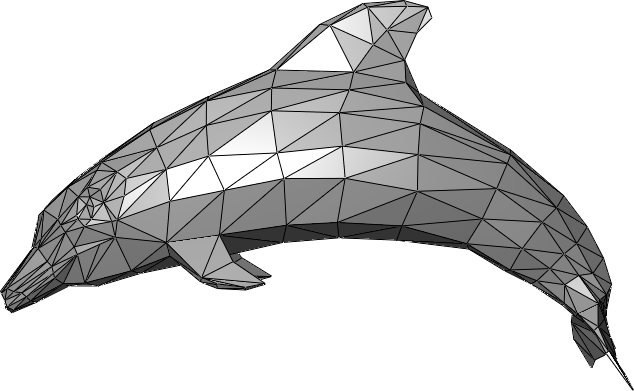
\includegraphics[width=\linewidth]{dolphin_mesh.png}
	\caption{A triangular mesh representing a dolphin \protect\cite{trianglemesh}.}\label{fig:dolphin mesh}
\end{wrapfigure}
Since we can intersect triangles now with our ray-triangle intersection. We can use the same method to load \textbf{triangular meshes}. A triangular mesh is a type of polygon mesh which comprises of a bunch of triangles. Just like a cube can be formed using 12 triangles (2 triangles for each face of the cube), you can create any 3D model with a bunch of triangles and the detail of the model depends on the amount of triangles the model has. The more the number of triangles in a mesh, the more accurately it can represent a model. Figure 12 shows an example of a triangular mesh of a dolphin. In the case of our ray tracer what we want to do is load all the triangles our mesh is made of, intersect all of those triangles using our ray-triangle intersection method and then compute the color of the points on all the triangles our ray intersects with. This is however an expensive process since many triangular meshes can comprise of thousands or even millions of triangles. The famous \textbf{Stanford Bunny} \cite{stanfordbunny} for example consists of about 69, 451 triangles. There are many methods to speed up the process of intersecting with complex objects, one of which would be discussed later in this report. The \textbf{normal} of a triangle would also play an important role in the next section when we move on to shade our meshes. For now, we can try to color our triangles with a constant color using their normals.
\\
\begin{figure}[H]
	\centering
	\captionsetup{justification=centering}
	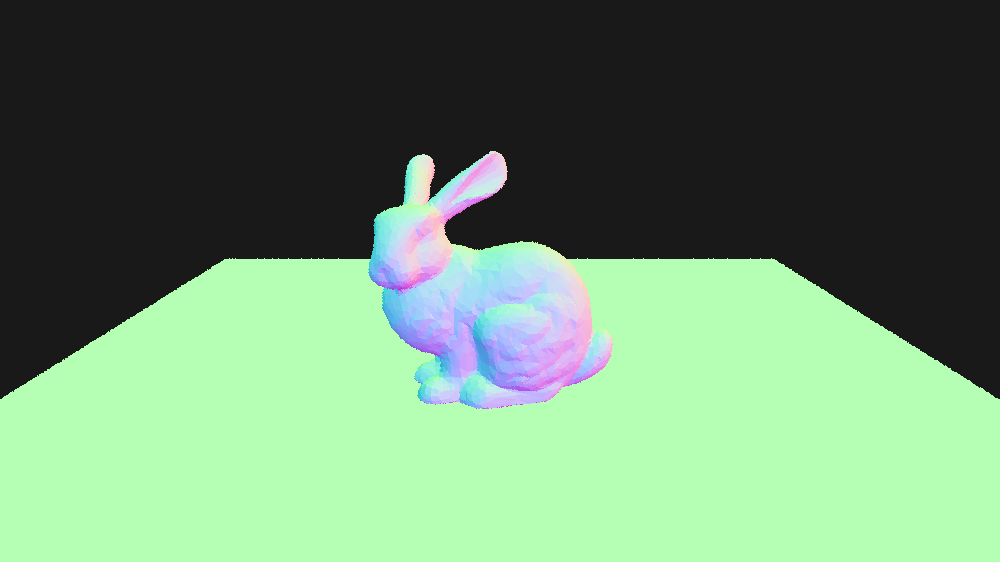
\includegraphics[width=0.54\textwidth]{normal_mesh.png}\quad
	\caption{Stanford Bunny on a plane visualized with constant colors according to normals. The one used here has 4, 968 triangles.}
\end{figure}

\endgroup

	\section{Shading}
	Now that we can do ray-sphere and ray-triangle intersections, we can implement some kind of shading. Shading refers to the process that gives visual appearance to objects in 3D space. Without shading, as you have observed in the image we generated previously, we can only show constant colors on our objects. But, what we really want to achieve is to show objects as close to how they look in real life. We would want glossy surfaces to look shiny while matte surfaces should look dull. What's needed to simulate materials of these kind, is some kind of \textbf{illumination}.
	\\~\\
	\textbf{Illumination} is a general term for light that originates at the light sources and arrives at object surfaces. Illumination can be divided into generally two types: Direct or Indirect. \textbf{Direct illumination} refers to the light that hits a surface directly from a light source while \textbf{indirect illumination} is the light that hits a surface after reflecting off from at least one surface. Direct illumination is also often referred to as \textbf{local illumination} while indirect illumination is referred to as \textbf{global illumination}. For the accompanied ray tracer, a well known local illumination model known as \textbf{Phong Illumination} model \cite{phong} has been implemented. It can simulate light as well as material shading. But it is important to discuss lights first, which would help us illuminate surfaces.
	\\~\\
	A light source in our scene is a virtual object that lets us illuminate other objects in our scene. A \textbf{light source} is defined with a \textbf{color} as well as \textbf{intensity}.
	\subsection{Point light}
	I have implemented \textbf{Point light} in my ray tracer which is a type of spherical light that emits light in all directions similar to a light bulb. They also only emit light from a single point in space. A point light's intensity reaching a point $\boldsymbol{p}$ on an object or anything in our scene also depends on how far the light is from that object. In fact, light source attenuation follows the \textbf{inverse square law} \cite{inversesquarelaw2} which states that a quantity (in our case, light intensity at a point) is inversely proportional to the square of the distance from source of the quantity (a light source). Or in other words, light intensity at a point $\boldsymbol{p}$ decreases quadratically with the distance from the light position $\boldsymbol{l}_{p}$. 
	\begin{figure}[H]
		\centering
		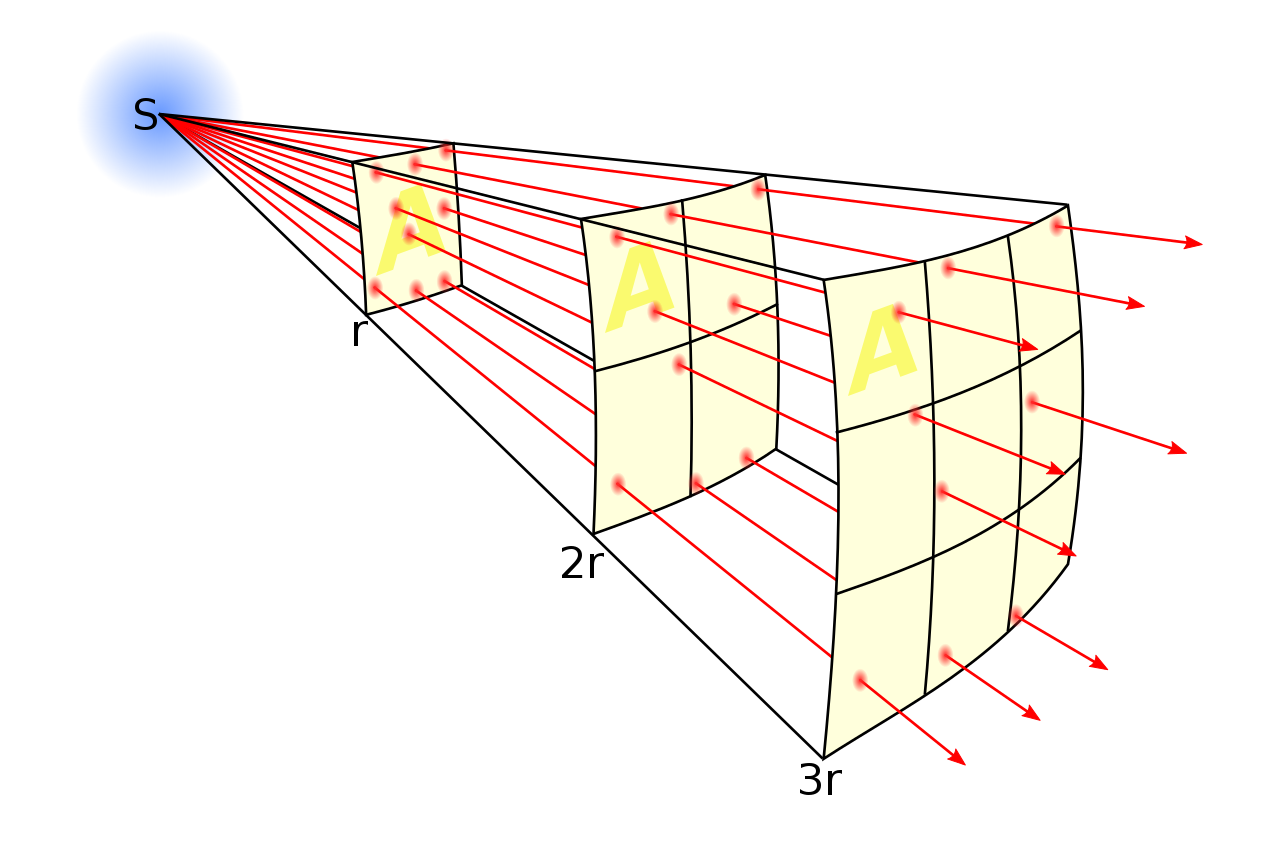
\includegraphics[width=.5\textwidth]{inverse_square_law.png}\quad
		\caption{Light's area grows quadratically with distance r \protect\cite{inversesquarelaw}.}
	\end{figure}
	\noindent For point lights, this can be formulated as:
	\begin{equation}
	l_{ip} = \frac{l_{i}}{4 * \pi * d^2}
	\end{equation}
	where $l_{ip}$ is the actual intensity reaching a point $\boldsymbol{p}$, $l_{i}$ is the intensity value of the light and $d$ is the distance between the light position $\boldsymbol{l}_{p}$ and point $\boldsymbol{p}$.
	\subsection{Diffuse Reflection} 
	
	\textbf{Diffuse reflection} simulates matte like surfaces. Surfaces that don't have shiny appearance and that reflect light in many directions. Surface illumination strength can be calculated by the dot product of the surface normal $\boldsymbol{n}$ and light source's direction $\boldsymbol{l}_{d}$ which is referred to as the \textbf{Lambert's Cosine Law} \cite{lambertscosinelaw}. In other words, illumination strength is directly proportional to the cosine of the angle between $\boldsymbol{n}$ and $\boldsymbol{l}_{d}$. If light intensity reaching a point $\boldsymbol{p}$ is given by $l_{ip}$ (as calculated above) and $\boldsymbol{\rho}$ is the albedo (hit point color) we can calculate the diffuse reflection at a point as:
	\begin{equation}
		\boldsymbol{l}_{diffuse} = \boldsymbol{\rho} * \frac{1}{\pi} * (\boldsymbol{n} \cdot \boldsymbol{l}_{d}) * \boldsymbol{l}_{color} * l_{ip}
	\end{equation}
	Where, $\boldsymbol{l}_{color}$ is the light's color. This can be done for multiple lights and the formula becomes:
	\begin{equation}
	\boldsymbol{l}_{diffuse} = \Sigma_{i} \boldsymbol{\rho} * \frac{1}{\pi} * (\boldsymbol{n} \cdot \boldsymbol{l}_{i_{d}}) * \boldsymbol{l}_{i_{color}} * l_{i_{ip}}
	\end{equation}
	So the total diffuse reflection $\boldsymbol{l}_{diffuse}$ reaching a point $\boldsymbol{p}$ is the sum of all the diffuse reflections calculated from all lights in the scene.
	\begin{figure}[H]
		\centering
		\captionsetup{justification=centering}
		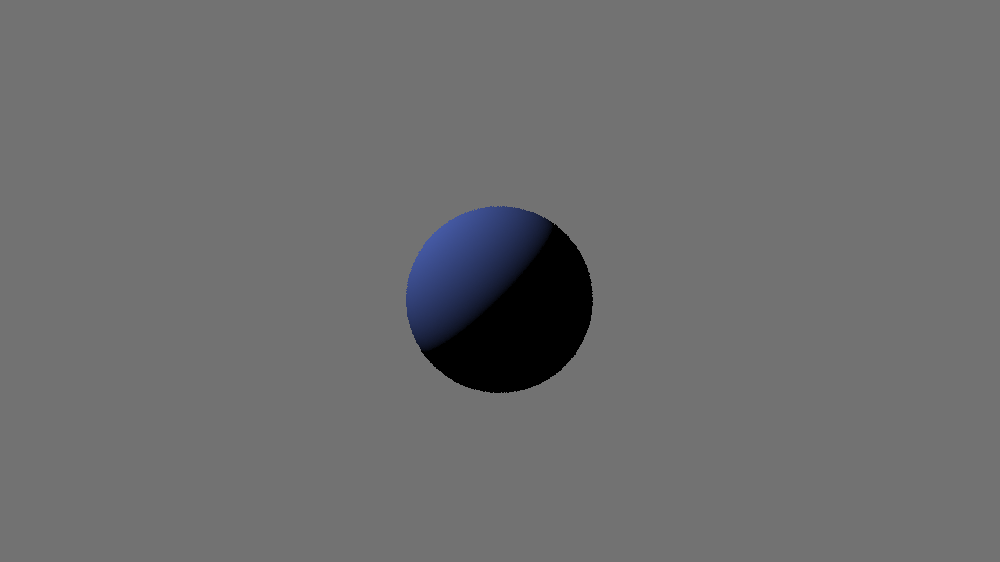
\includegraphics[width=0.5\textwidth]{diffuse_reflection.png}\quad
		\caption{A blue sphere with a point light at top-left.}
	\end{figure}

	\subsection{Ambient Reflection}
	\textbf{Ambient Reflection} can be described as indirect illumination from other surfaces. In the accompanied ray tracer, the albedo of the surface is being used as the ambient value. This can also be multiplied with a constant $k_{amb}$ to increase or decrease the ambient intensity. Overall, ambient reflection can be given as:
	\begin{equation}
	\boldsymbol{l}_{ambient} = \boldsymbol{\rho} * k_{amb}
	\end{equation}
	Combining our diffuse and ambient components, our formula for an individual point light becomes:
	\begin{equation}
	\boldsymbol{l}_{total} = (\boldsymbol{\rho} * k_{amb}) + \boldsymbol{\rho} * \frac{1}{\pi} * (\boldsymbol{n} \cdot \boldsymbol{l}_{d}) * \boldsymbol{l}_{color} * l_{ip}
	\end{equation}
	\begin{figure}[H]
		\centering
		\captionsetup{justification=centering}
		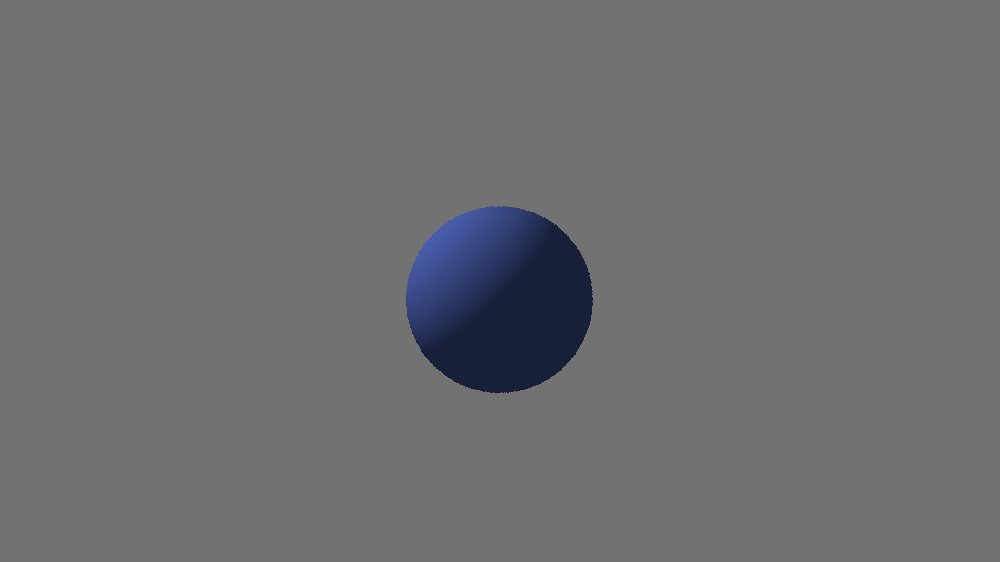
\includegraphics[width=0.5\textwidth]{diffuse_ambient_reflection}\quad
		\caption{A blue sphere with a point light at top-left.}
	\end{figure}

	\subsection{Specular Reflection}
	\begin{wrapfigure}{r}{0.40\textwidth}
		\centering
		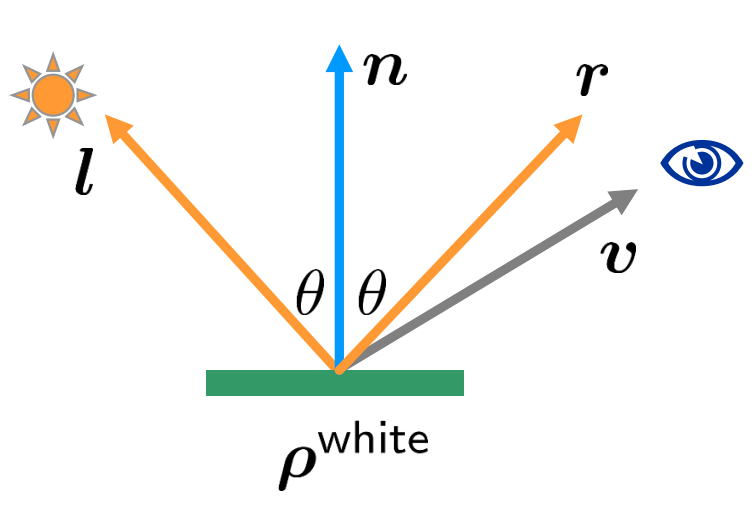
\includegraphics[width=0.65\linewidth]{r_vector_v_vector} 
		\caption{Reflection vector $\boldsymbol{r}$, view vector $\boldsymbol{v}$ and other useful vectors \protect\cite{shadinglecture}.}
		\label{fig:wrapfig}
	\end{wrapfigure}
	\textbf{Specular Reflection} simulates shiny surfaces. These kind of surfaces reflect light in some dominant directions instead of diffuse which reflects light in all directions. For producing specular highlights, we need a reflection vector $\boldsymbol{r}$ which is the reflected light from a shiny surface. This can be calculated as:
	\begin{equation}
	\boldsymbol{r} = 2 * (\boldsymbol{l} \cdot \boldsymbol{n}) * \boldsymbol{n} - \boldsymbol{l}
	\end{equation}
	where vectors $\boldsymbol{l}$ and $\boldsymbol{n}$ are light direction and surface (hit) normal respectively. Both of these vectors should be normalized. After calculating the reflection vector, we need to calculate the view vector $\boldsymbol{v}$ which is the vector from the surface point $\boldsymbol{p}$ to the ray origin $\boldsymbol{r_{o}}$. After calculating both these vectors, the specular value of a surface point can then be calculated as:
	\begin{equation}
	\boldsymbol{l}_{specular} = \boldsymbol{l}_{color} * (\boldsymbol{r} \cdot \boldsymbol{v})^m * k_{spec}
	\end{equation}
	where $m$ is sometimes called the \textbf{shininess} constant. We can get different specular highlights for different values of $m$. Overall reflected light depends on $m$. $k_{spec}$ is just a constant to have the desired amount of specular reflection for a surface. Combining diffuse, ambient and specular gives us this formula for an individual point light:
	\begin{equation}
	\boldsymbol{l}_{total} = (\boldsymbol{\rho} * k_{amb}) + \boldsymbol{\rho} * \frac{1}{\pi} * (\boldsymbol{n} \cdot \boldsymbol{l}_{d}) * \boldsymbol{l}_{color} * l_{ip} + \boldsymbol{l}_{color} * (\boldsymbol{r} \cdot \boldsymbol{v})^m * k_{spec}
	\end{equation}
	\begin{figure}[H]
		\centering
		\captionsetup{justification=centering}
		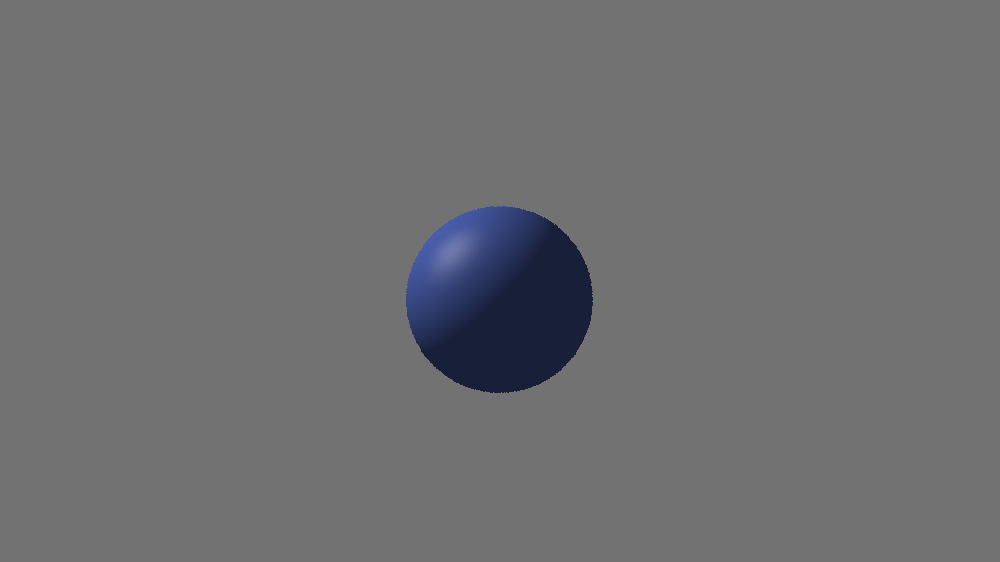
\includegraphics[width=0.5\textwidth]{diffuse_ambient_specular_reflection}\quad
		\caption{A blue sphere with a point light at top-left. For this render, $k_{amb}$ was $0.05$, $m$ was $10$, $k_{spec}$ was $0.1$ and $\boldsymbol{l}_{color}$ was $(1, 1, 1)$ with $l_{ip}$ of 30.}
	\end{figure}

	\section{Shadows}
	
	For adding shadows in our scene, we need to compute an additional ray from the point of surface where our ray hits $\boldsymbol{p}$ towards the light position $\boldsymbol{l}_{p}$. If this ray which is often called as \textbf{shadow ray} hits another object on its way towards the light source, then the point that we are shading is in the shadow of that object. \\~\\We have to be careful though when we try to find out if a hit point $\boldsymbol{p}$ is in shadow of an object and we only have to check the hit points which are between the point being shaded and the light location otherwise we can have an issue as shown below: 
	
	\begin{figure}[H]
		\centering
		\captionsetup{justification=centering}
		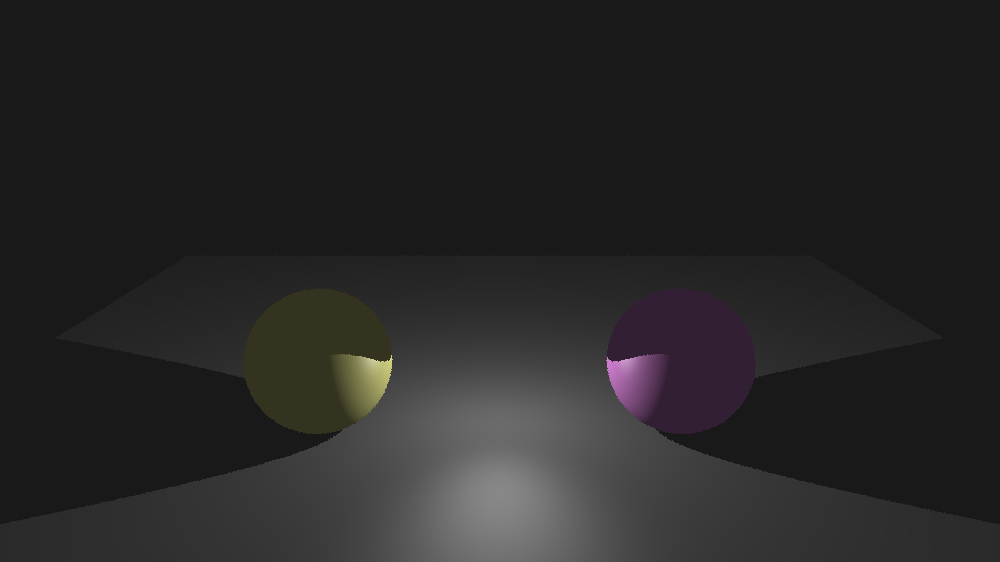
\includegraphics[width=0.5\textwidth]{shadow_ray_problem.png}\quad
		\caption{A point light between two spheres creates unexpected shadows on spheres.}
	\end{figure}
	
	\noindent
	Note the unexpected shadow that appears on both of these spheres. As we try to compute a shadow ray on a point on the yellow sphere, our ray (from hit point $\boldsymbol{p}$ towards $\boldsymbol{l}_{p}$) goes beyond the light position and hits the pink sphere on the right side of the light and since it hit an object, we assume the point we were shading on the yellow sphere is in the shadow of an object while it actually isn't. The same happens with the pink sphere and we get an unexpected shadow. We can fix this by only testing our shadow ray between the position of our hit point $\boldsymbol{p}$ and the light position $\boldsymbol{l}_{p}$ after which we get the desired image as shown in figure 20.
	\\
	\begin{figure}[H]
		\centering
		\captionsetup{justification=centering}
		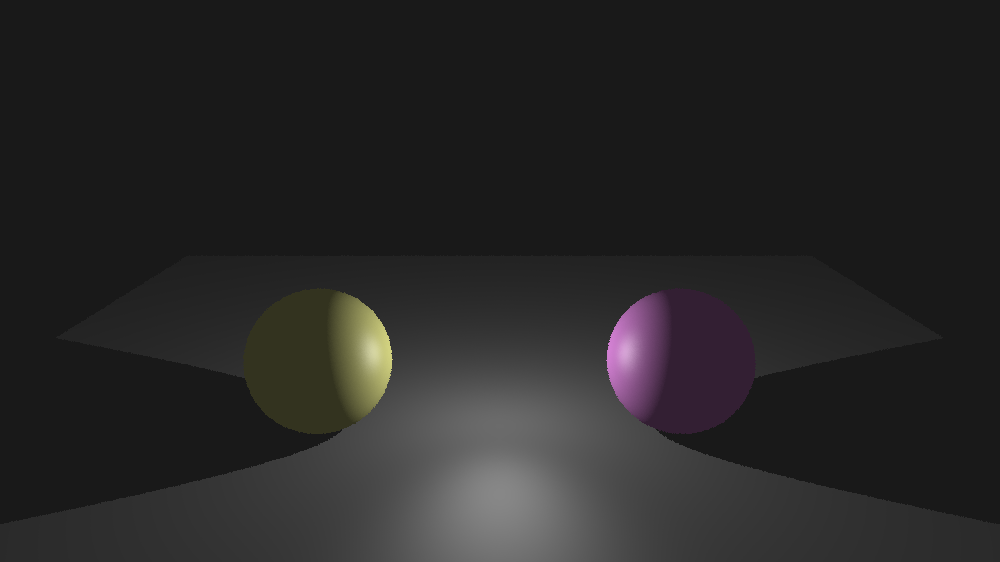
\includegraphics[width=0.5\textwidth]{shadow_ray_problem_fix.png}\quad
		\caption{A point light between two spheres.}
	\end{figure}
	
	\noindent
	\\
	One another problem that often arises due to finite floating point precision is \textbf{shadow acne} or \textbf{salt and pepper noise}. The reason why that happens is due to the fact that when shadow rays intersect with an object, it is assumed that the hit function will return a value of $0$ for $t$ but that is not always the case. Sometimes, due to finite numerical precision, this $t$ can be slightly positive $(3.245e-07)$ or slightly negative $(-4.567e-08)$ and these positive values are what causes the issue because then our hit function returns \textbf{true} and the shadow ray intersects the object where it was being cast. This can be fixed by introducing a small bias value and moving the shadow ray a bit towards the surface normal. The accompanied ray tracer uses a bias value of $0.001$ so the shadow ray's origin becomes:
	\begin{equation}
		\boldsymbol{r}_{o} = \boldsymbol{p}_{hit} + \boldsymbol{n}_{hit} * 0.001
	\end{equation}
	where $\boldsymbol{p_{hit}}$ is the hit position and $\boldsymbol{n_{hit}}$ is the hit normal.
	
	\section{Antialiasing}
	So far the images we have produced have sharp jaggy edges. This is not so obvious if we look the image as a whole but still noticeable if the image is zoomed in a little.
	\begin{figure}[H]
		\centering
		\captionsetup{justification=centering}
		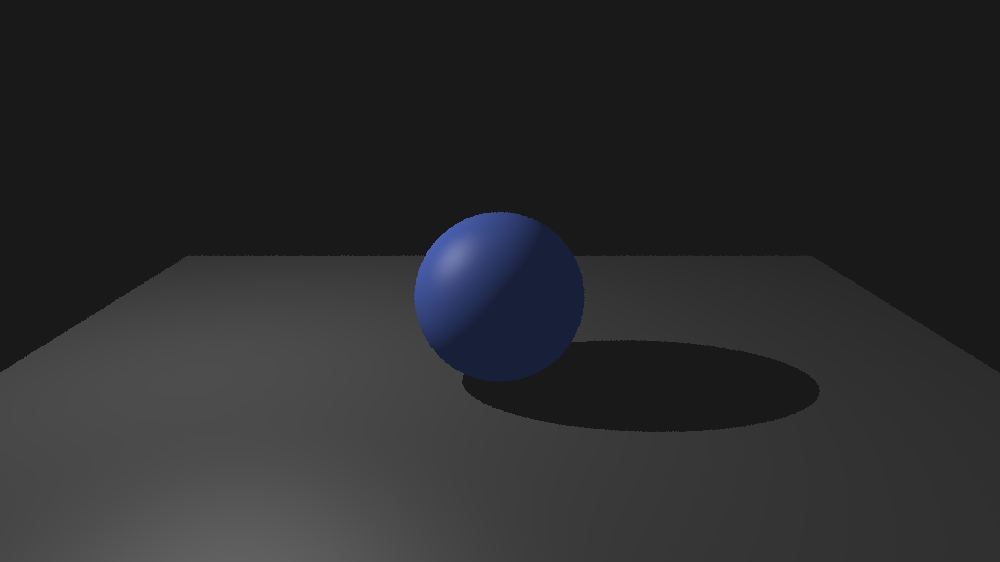
\includegraphics[width=.45\textwidth]{aliased_pointlight.png}\quad
		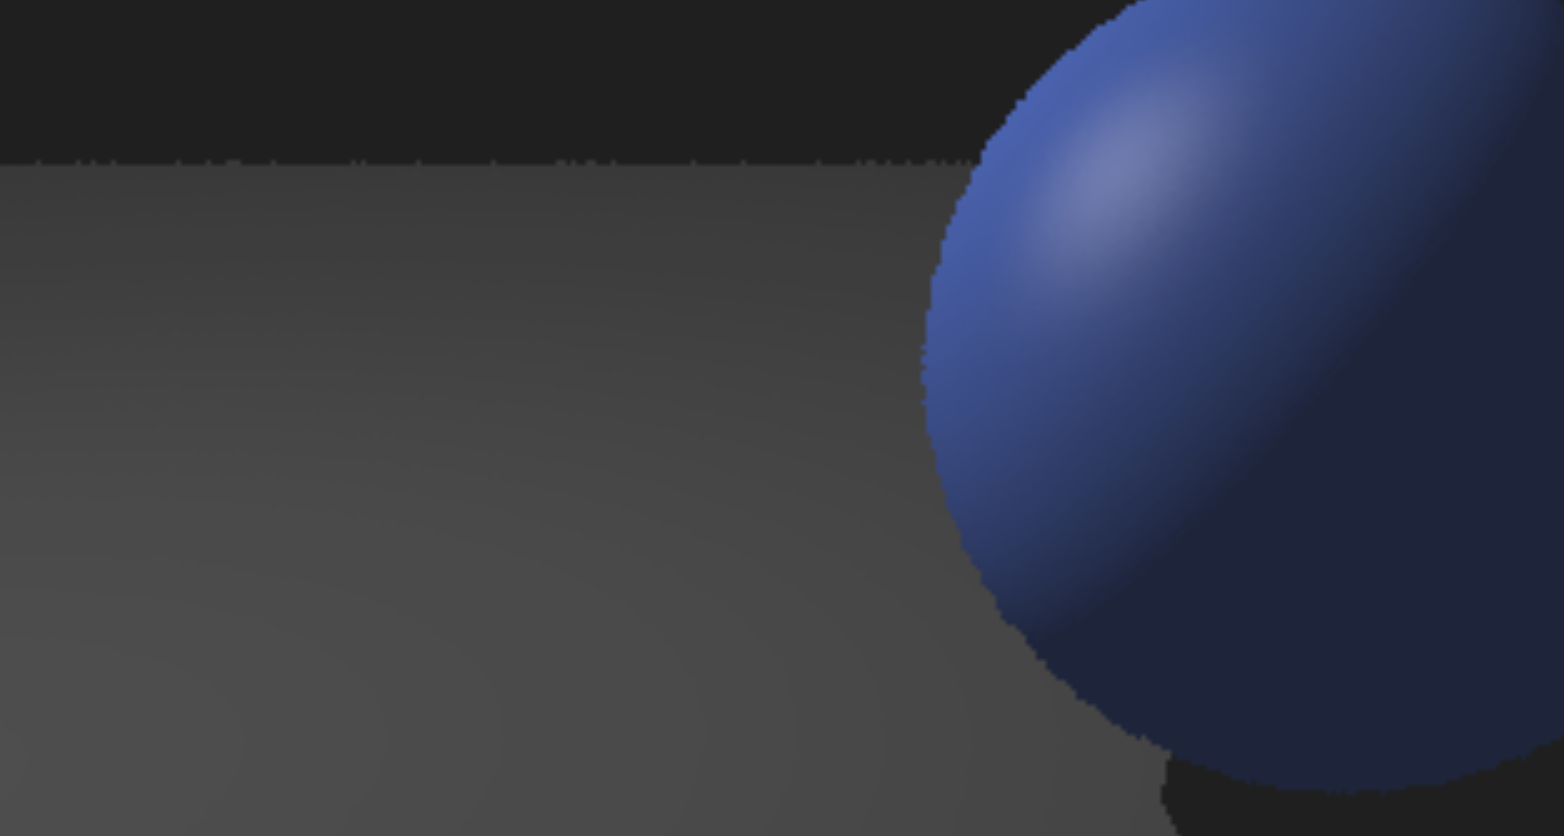
\includegraphics[width=.47\textwidth]{aliased_pointlight_zoomed.png}\quad
		\caption{Image rendered has sharp and jaggy edges.}
	\end{figure}
	\noindent
	This is because we are only sending one ray per pixel from its center. Considering an image with width 6 pixels and height 5 pixels where a ray is sent to the center of the pixel can be shown as:
	\begin{figure}[H]
		\centering
		\captionsetup{justification=centering}
		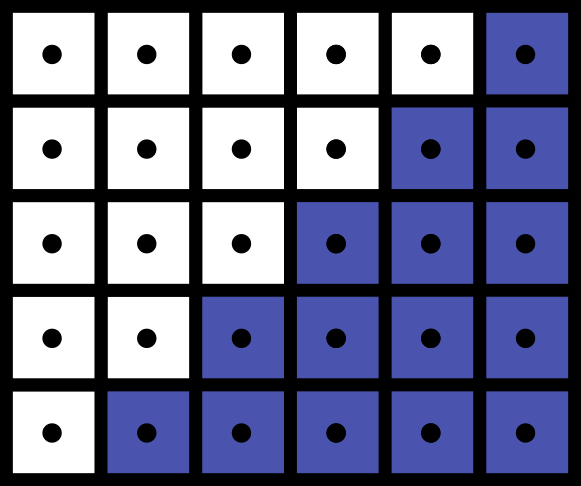
\includegraphics[width=0.25\textwidth]{antialiasing_1.png}\quad
		\caption{A 6x5 image where a ray is sent to the center of the pixel \protect\cite{suffern2016ray}.}
	\end{figure}
	\noindent
	But what we really want is an image like the one shown below, where the transition between colored pixels is smooth and not pixelated:
	\begin{figure}[H]
		\centering
		\captionsetup{justification=centering}
		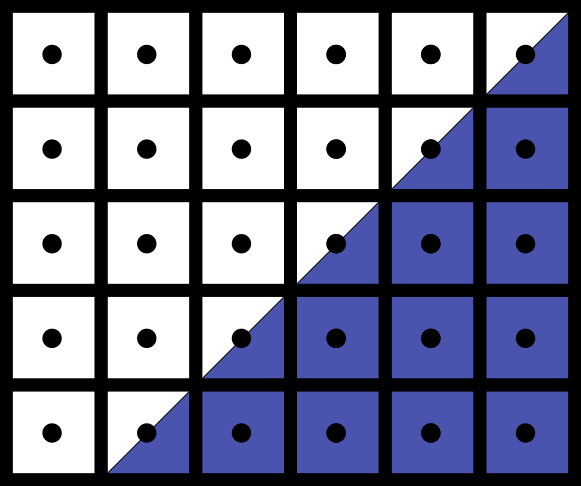
\includegraphics[width=0.25\textwidth]{antialiasing_2.png}\quad
		\caption{Desired image. \protect\cite{suffern2016ray}.}
	\end{figure}

	\noindent
	One way to achieve this is by sending multiple rays per pixel instead of just one. The ray tracer accompanied with this report sends multiple rays per pixel with a random range between $[0, 1)$ according to the desired amount of \textbf{anti aliasing} set. The color of all those rays are accumulated and then divided by the number of samples per pixel. So if we sent 10 rays per pixel, the returned colors of all those rays are added and then divided by 10. Note that for 10x anti aliasing, since we are sending 10 rays per pixel, this has also increased our time complexity by 10x so if we were sending 25 rays for a 5x5 image, now we are sending 250 rays for the same image.
	
	\begin{figure}[H]
		\centering
		\captionsetup{justification=centering}
		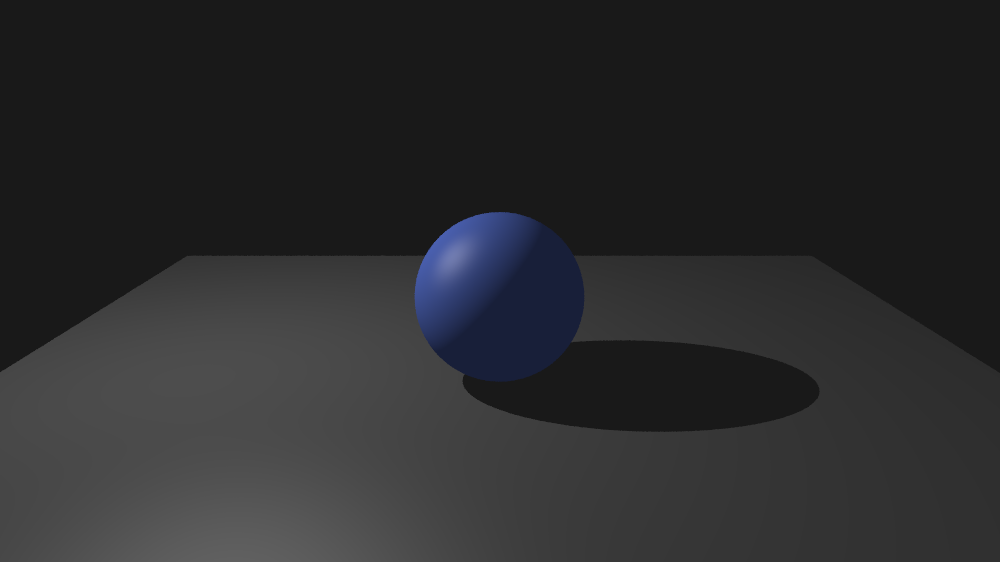
\includegraphics[width=.45\textwidth]{antialiased_pointlight.png}\quad
		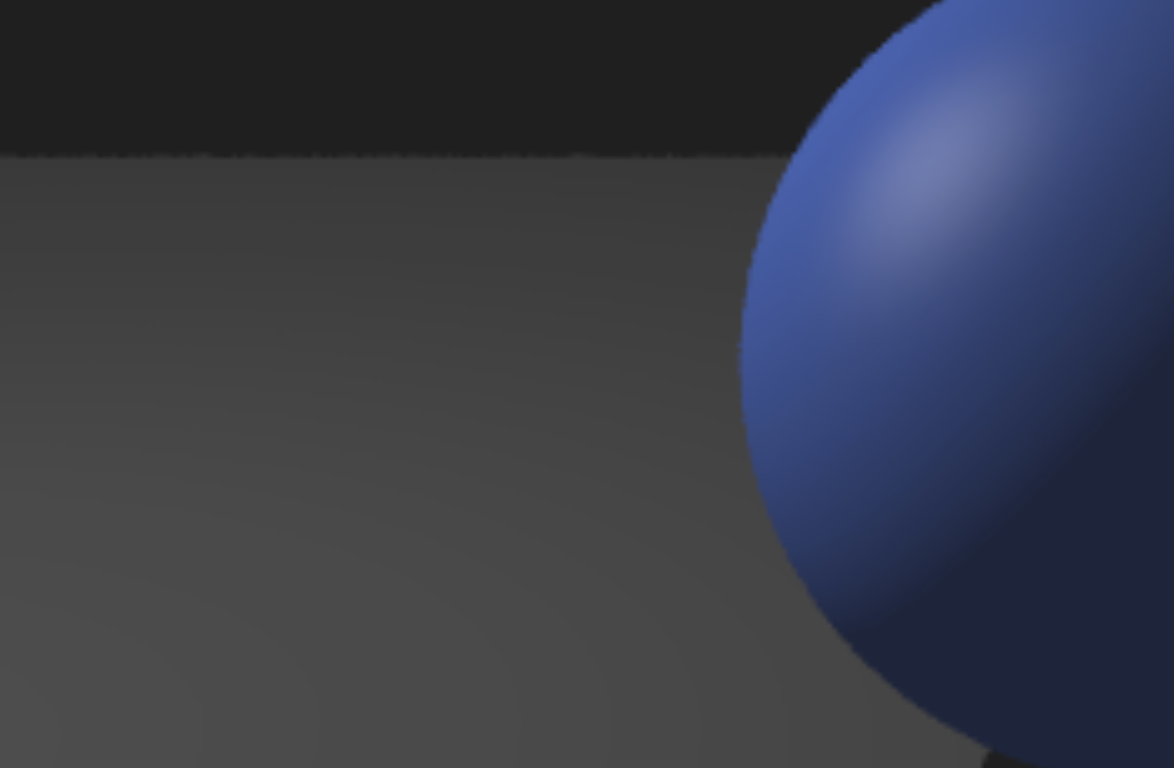
\includegraphics[width=.39\textwidth]{10x_antialiasing.png}\quad
		\caption{Image rendered with 10x anti aliasing.}
	\end{figure}

	\section{Texture mapping}
	
	\textbf{Texture mapping} is exactly what the term says. We have a texture, which can be any image of variable size and we want to map this image to a 3D object in our scene. An image's pixel is often represented as $(u, v)$ coordinates that go from $0$ to $1$. If we have a grass texture for example, we can map the image to $(u, v)$ coordinates as:
	\begin{figure}[H]
		\centering
		\captionsetup{justification=centering}
		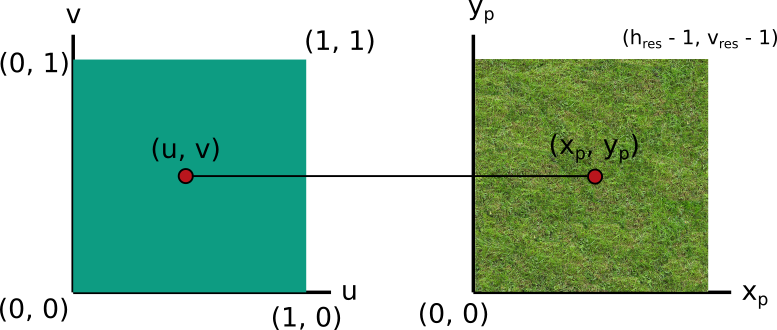
\includegraphics[width=.7\textwidth]{texture_mapping.png}\quad
		\caption{$(u, v)$ coordinates being mapped from an image with resolution $h_{res}*v_{res}$ \protect\cite{suffern2016ray}.}
	\end{figure}
	\noindent
	Here, we have a texture image with horizontal resolution or width represented as $h_{res}$ and vertical resolution or height represented as $v_{res}$. And the mapping from $(u, v)$ to $(x_{p}, y_{p})$ can be given as:
	\begin{equation}
		x_{p} = (h_{res} - 1)*u
	\end{equation}
	\begin{equation}
		y_{p} = (v_{res} - 1)*v
	\end{equation}
	
	\subsection{Texturing background}
	Texturing our background is as simple as copying a pixel from the texture to our image that is being rendered. Since, we are going pixel by pixel as we render the image, we take the pixel's row and column number and divide it by width and height respectively, which gives us the $(u, v)$ coordinate:
	\begin{equation}
		u = \frac{pixel_{r}}{image_{w}}
	\end{equation}
	\begin{equation}
		v = \frac{pixel_{c}}{image_{h}}
	\end{equation}
	\noindent
	Where, $pixel_{r}$ is the pixel's row value, $pixel_{c}$ is the pixel's column value, $image_{w}$ is the width of the image being rendered and $image_{h}$ is the height of the image being rendered. So if we are rendering an image of width $1000$ and height $562$ and want to determine the texture value for pixel $(500, 286)$, we get $(u, v)$ as $(0.5, 0.508)$. We can then use this $(u, v)$ coordinate and equations (28) and (29) to get the pixel value from our texture.
	
	\subsection{Texturing a triangle}
	Texturing a triangle is also fairly easy. The algorithm we used for our ray-triangle intersection, computes $t$, $\alpha$ and $\beta$ where $\alpha$ and $\beta$ are actually two of the three \textbf{barycentric coordinates} of our triangle. These can be used to texture map our triangle, as barycentric coordinates essentially linearly interpolate between the three vertices of a triangle. Using $\alpha$ as $u$ and $\beta$ as $v$, we can use equation $(28)$ and $(29)$ to get the desired pixel from the texture and then use the pixel's $(r, g, b)$ value as the albedo $(\boldsymbol{\rho})$ of our hit point on our triangle. Using the grass texture on two triangles making a plane gives us an image:
	\begin{figure}[H]
		\centering
		\captionsetup{justification=centering}
		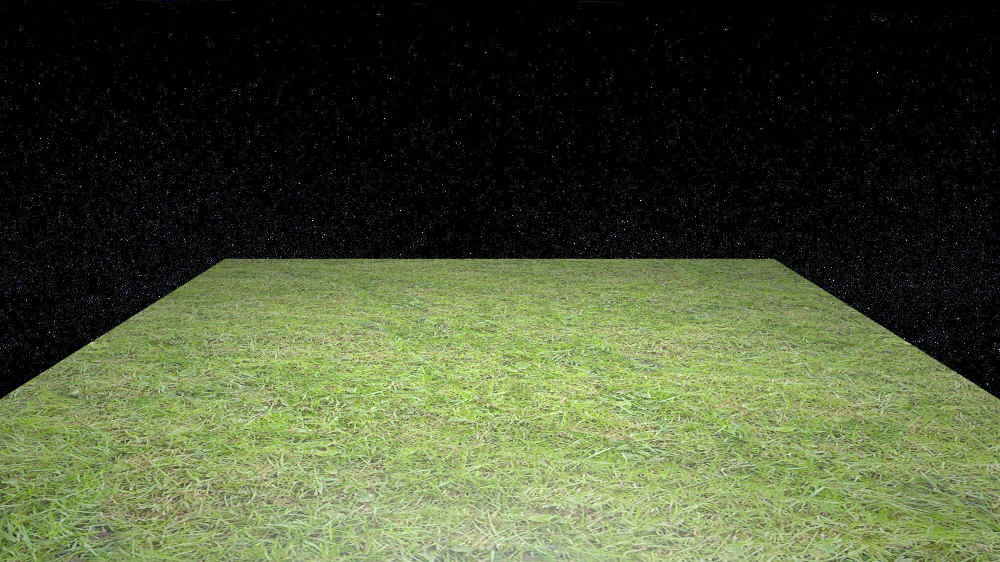
\includegraphics[width=.5\textwidth]{textured_triangles.png}\quad
		\caption{Two textured triangles making a plane, with three point lights illuminating the scene. A stars texture is used as a background.}
	\end{figure}

	\noindent
	Note: Textures for meshes were not implemented due to time constraints.

	\subsection{Texturing a sphere}
	\begingroup
	\setlength{\intextsep}{5pt}
	\setlength{\columnsep}{35pt}
	\begin{wrapfigure}{r}{0.45\textwidth}
		\centering
		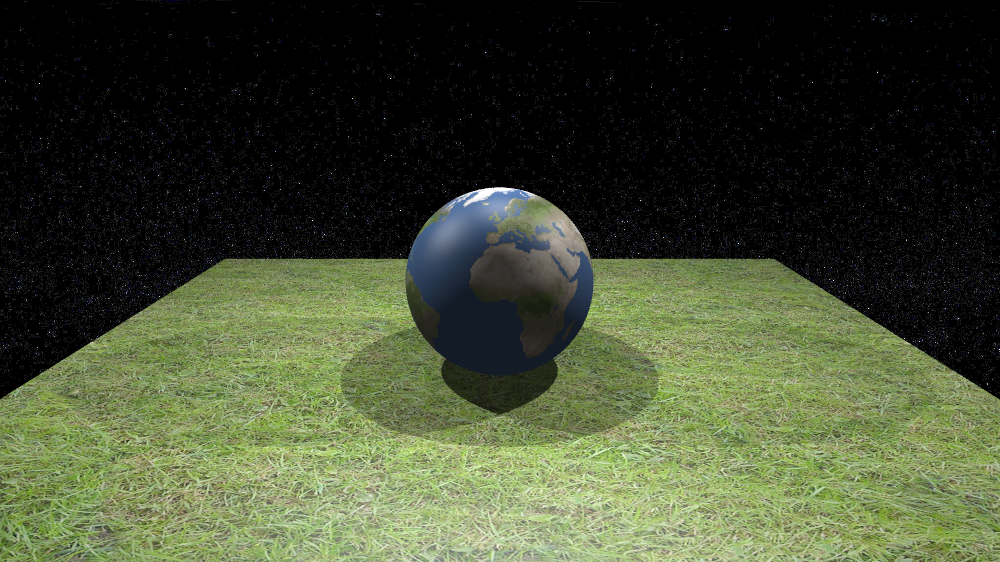
\includegraphics[width=\linewidth]{textured_sphere.png}
		\caption{Two textured triangles making a plane, a sphere with an earth texture in the middle with three point lights illuminating the scene. A stars texture is used as a background.}\label{fig:textured_sphere}
	\end{wrapfigure}
	In order to texture map a sphere, we need to compute the $(u, v)$ coordinates since we are not calculating them as part of our ray-sphere intersection algorithm. Just to review, our ray-sphere intersection returns a root $t$ which is the scalar we use to get the hit position on our sphere using:
	\begin{equation}
	\boldsymbol{p_{hit}} = \boldsymbol{o} + t*\boldsymbol{d} 
	\end{equation}
	where $\boldsymbol{o}$ is ray origin and $\boldsymbol{d}$ is the ray direction. After getting the hit position $\boldsymbol{p_{hit}}$ we get the normal on our sphere by:
	\begin{equation}
	\boldsymbol{{n}} = \frac{\boldsymbol{p_{hit}} - \boldsymbol{c}}{r}
	\end{equation}
	where $\boldsymbol{c}$ is the center of our sphere and $r$ is the radius. A sphere has smooth normals on every point which means that $\boldsymbol{n}$ would be different for every $\boldsymbol{p_{hit}}$. Once we have computed $\boldsymbol{n}$, we can get the $(u, v)$ coordinates for the sphere that would help us map a texture to our sphere:
	\begin{equation}
	u = 0.5 + \frac{arctan2(n_{x}, n_{z})}{2 * \pi}
	\end{equation}
	\begin{equation}
	v = 0.5 - \frac{arcsin(n_{y})}{\pi}
	\end{equation}
	where $n_{x}, n_{y}, n_{z}$ are the $x, y$ and $z$ coordinates of the normal $\boldsymbol{n}$. Using equations $(34)$ and $(35)$ for $(u, v)$ coordinates of our sphere, we can then use equations $(28)$ and $(29)$ to get the desired pixel from our texture.
	\endgroup
	\section{Transformations}
	It would be convenient to translate, scale and rotate objects in our scene. In order to create complex scenes with lots of geometries, scattered all over our scene, it is useful to have some kind of transformation operations on our objects so that we can translate, scale or rotate them according to our needs. This is often done by the help of \textbf{affine transformations} which we will discuss one by one.
	\subsection{Translation}
	\begin{wrapfigure}{r}{4cm}
		\centering
		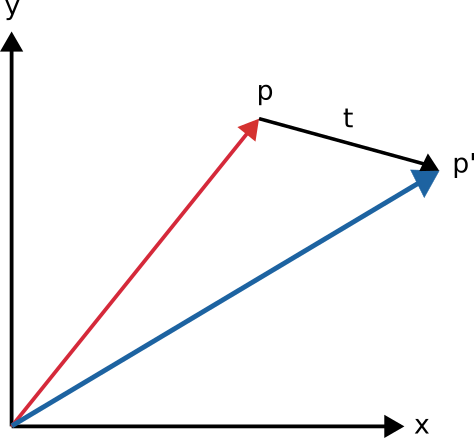
\includegraphics[width=4cm, height=4cm]{translation} 
		\caption{A vector $\boldsymbol{p}$ is translated using a vector $\boldsymbol{t}$ resulting in a vector $\boldsymbol{p'}$ \protect\cite{2dtransformations}.}
		\label{fig:scale}
	\end{wrapfigure}
	We will discuss \textbf{translation} first. This helps us moving objects in our scene to a particular position. This can be illustrated in 2D using vectors as shown in figure 28.
	\noindent
	In the figure, we have a vector $\boldsymbol{p}$ which is translated using a vector $\boldsymbol{t}$ resulting in a vector $\boldsymbol{p'}$. This is essentially vector addition and can be given by:
	\begin{equation}
	\boldsymbol{p'} = \boldsymbol{p} + \boldsymbol{t}
	\end{equation}
	Note that for 3D, we must have an added dimension $z$ in our vector. The above figure was just to make it simple to illustrate. In the case of a sphere, we will be applying this vector addition to its center, $\boldsymbol{c}$ and in the case of a triangle we will be doing this operation to each of its vertices $\boldsymbol{v_{0}}$, $\boldsymbol{v_{1}}$ and $\boldsymbol{v_{2}}$. For meshes, this has to be done for each of the triangles' vertices in a mesh. 
	\subsection{Scale}
	
	\begin{wrapfigure}{r}{4cm}
		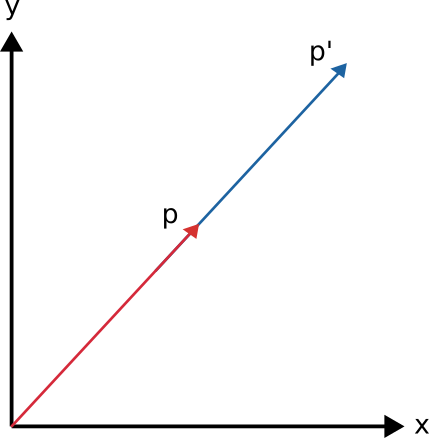
\includegraphics[width=4cm,height=4cm]{scale} 
		\caption{A vector $\boldsymbol{p}$ is scaled to a resulting vector $\boldsymbol{p'}$ \protect\cite{2dtransformations}.}
		\label{fig:scale}
	\end{wrapfigure}
	We would also like to \textbf{scale} objects in our scene. This helps changing the size of our objects, whether they are spheres or meshes. Each mesh also has a fixed size in their original format (.obj for example) and without scaling we won't be able to change its size. Scaling can be illustrated in 2D using vectors as shown in figure 29. We have a vector $\boldsymbol{p}$ which have been scaled to a vector $\boldsymbol{p'}$. Note that the vector is scaled in both $x$ and $y$ direction with the same amount which is also called \textbf{uniform scaling}. So essentially scaling is multiplication of a vector with a scaling factor $s$ which can be given by:
	\begin{equation}
	\boldsymbol{p'} = \boldsymbol{p}*s
	\end{equation}
	We can also do \textbf{non uniform scaling} by using a different scaling factor for each of the $x$, $y$ and $z$ coordinates of our vector. Which means that we want to scale our dimensions non uniformly. This can be given as:
	\begin{equation}
	p'_{x} = p_{x}*s_{x}
	\end{equation}
	\begin{equation}
	p'_{y} = p_{y}*s_{y}
	\end{equation}
	\begin{equation}
	p'_{z} = p_{z}*s_{z}
	\end{equation}
	In the case of a sphere, scaling is multiplication of a scaling factor $s$ with its radius $r$ and in the case of a triangle it is the multiplication of a scaling factor with each of its vertices.
	
	\subsection{Rotation}
	\textbf{Rotation} is also useful since there will always be a need to rotate objects in our scene. Rotation in 2D using vectors can be illustrated as:
	\begin{figure}[H]
		\centering
		\captionsetup{justification=centering}
		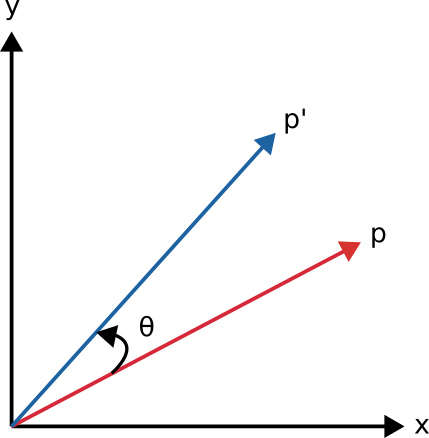
\includegraphics[width=.28\textwidth]{rotation.png}\quad
		\caption{A vector $\boldsymbol{p}$ is rotated by an angle $\theta$ resulting in a vector $\boldsymbol{p'}$ \protect\cite{2dtransformations}.}
	\end{figure}
	\noindent
	In 2D you can only rotate in clockwise or anti-clockwise direction. This can be thought of placing a paper on a table and then trying to rotate it without lifting it. And you quickly notice that it can only be done in clockwise or anti-clockwise manner. Anti-clockwise rotation in 2D which is the same shown in figure 30 can be given by:
	\begin{equation}
	p'_{x} = p_{x}*(cos\theta) + p_{y}*(-sin\theta)
	\end{equation}
	\begin{equation}
	p'_{y} = p_{x}*(sin\theta) + p_{y}*(cos\theta)
	\end{equation}
	For clockwise rotation this becomes:
	\begin{equation}
	p'_{x} = p_{x}*(cos\theta) + p_{y}*(sin\theta)
	\end{equation}
	\begin{equation}
	p'_{y} = p_{x}*(-sin\theta) + p_{y}*(cos\theta)
	\end{equation}
	But since, we are working in 3D, we need to be able to rotate at any axis. Rotation in 3D can be done in $x$, $y$ or $z$ axis or can also be a combination of rotation around these axis. Rotation around $x$ axis is given by:
	\begin{equation}
	p'_{x} = p_{x}
	\end{equation}
	\begin{equation}
	p'_{y} = p_{y}*(cos\theta) + p_{z}*(sin\theta)
	\end{equation}
	\begin{equation}
	p'_{z} = p_{y}*(-sin\theta) + p_{z}*(cos\theta)
	\end{equation}
	Rotation around $y$ axis is given by:
	\begin{equation}
	p'_{x} = p_{x}*(cos\theta) + p_{z}*(-sin\theta)
	\end{equation}
	\begin{equation}
	p'_{y} = p_{y}
	\end{equation}
	\begin{equation}
	p'_{z} = p_{x}*(sin\theta) + p_{z}*(cos\theta)
	\end{equation}
	And rotation around $z$ axis is given by:
	\begin{equation}
	p'_{x} = p_{x}*(cos\theta) + p_{y}*(sin\theta)
	\end{equation}
	\begin{equation}
	p'_{y} = p_{x}*(-sin\theta) + p_{y}*(cos\theta)
	\end{equation}
	\begin{equation}
	p'_{z} = p_{z}
	\end{equation}
	
	\pagebreak
	\section{Camera}
	
	\begin{wrapfigure}{r}{0.5\textwidth}
		\centering
		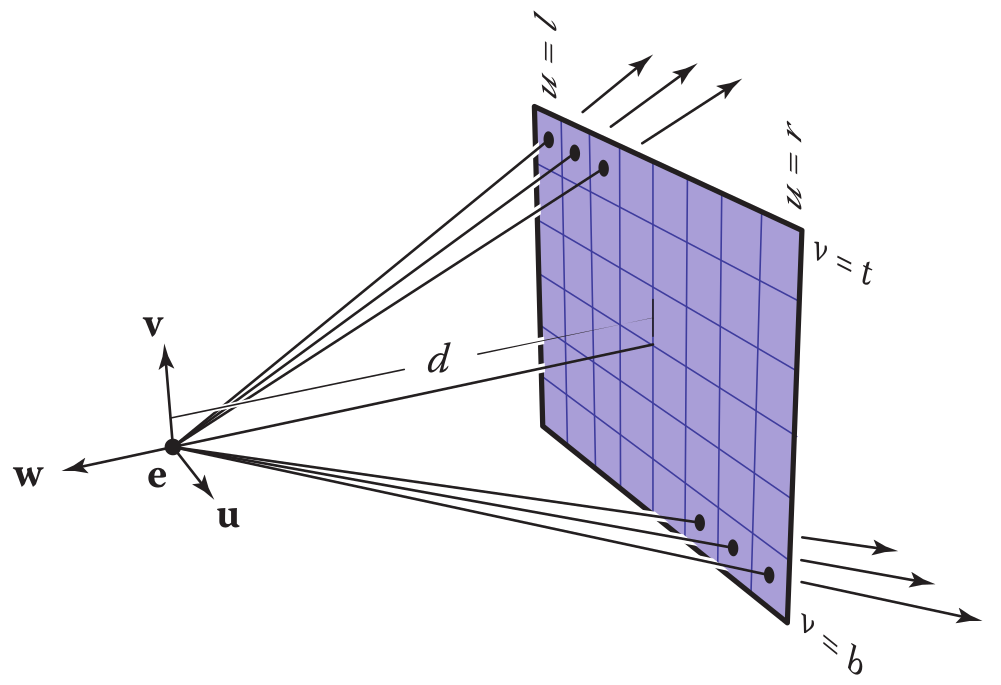
\includegraphics[width=0.8\linewidth]{camera_rays} 
		\caption{A visualization of a perspective view. The rays start at the viewpoint $\boldsymbol{e}$ and go through each of the pixels in an image. \protect\cite{marschner2018fundamentals}.}
		\label{fig:wrapfig2}
	\end{wrapfigure}
	
	The \textbf{camera} in a ray tracer is the point where the rays start and go through each pixel. The accompanied ray tracer uses a virtual pinhole camera which implements perspective viewing. A perspective view, shows a scene the way it should look when a human sees it. Objects that are far should appear smaller and objects that are closer to the camera should appear bigger. This type of camera also gives more information about depth. The setting that is used in the ray tracer can best be visualized by figure 31.
	For a perspective view, all the rays have the same origin, which is at the viewpoint $\boldsymbol{e}$. The directions however, are different for each pixel. The image plane is at some distance $d$ in front of $\boldsymbol{e}$. This distance is often also known as the \textbf{focal length} of a camera. It is important to mention \textbf{field of view (fov)} of the camera here. This is the extent of the virtual scene observed through the camera. 
	\begin{figure}[H]
		\centering
		\captionsetup{justification=centering}
		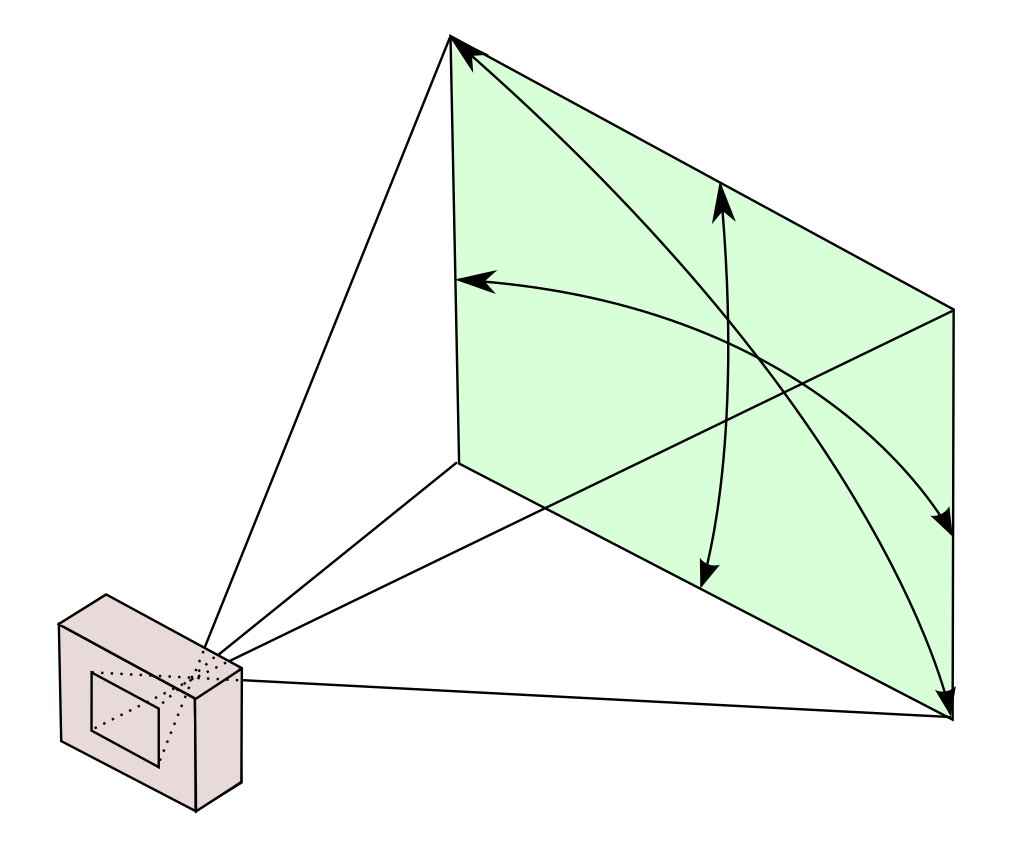
\includegraphics[width=.25\textwidth]{fov.png}\quad
		\caption{Field of view of a camera \protect\cite{fieldofview}.}
	\end{figure}
	\noindent
	As we move our camera, forwards or backwards (changing our z-axis), we need to be careful that the field of view is used to calculate a scaling factor for our view-port height and width. This scaling factor $h$ is calculated as:
	\begin{equation}
		h = tan\left(\frac{\theta}{2}\right)
	\end{equation}
	\noindent
	where $\theta$ is our field of view angle specified in radians. Our view-port width and height can then be calculated as:
	\begin{equation}
		view_{h} = 2 * h
	\end{equation}
	\begin{equation}
	view_{w} = aspect_{r} * view_{h}
	\end{equation}
	\noindent
	where $aspect_{r}$ is the aspect ratio of the image and is typically kept at 16:9. We also need a way to specify a position to look from ($\boldsymbol{e}$) so that we can view our scene from any point and a position to look at ($\boldsymbol{l}$) so that the focus of our camera is on a specific point in a scene. This is achieved using an orthonormal basis (ONB) represented as ($\boldsymbol{u, v, w}$) which can also be seen in figure 31 above. The vector $\boldsymbol{w}$ of the ONB is calculated as:
	\begin{equation}
		\boldsymbol{w} = \frac{\boldsymbol{e} - \boldsymbol{l}}{||\boldsymbol{e} - \boldsymbol{l}||}
	\end{equation}
	\noindent
	where $\boldsymbol{e}$ is the position we are looking from and $\boldsymbol{l}$ is the position we are looking at. The second vector $\boldsymbol{u}$ is calculated as:
	\begin{equation}
		\boldsymbol{u} = \frac{\boldsymbol{up} \times \boldsymbol{w}}{||\boldsymbol{up} \times \boldsymbol{w}||}
	\end{equation}
	where $\boldsymbol{up}$ is the up-vector usually taken as $(0, 1, 0)$ i.e y-axis. The third vector $\boldsymbol{v}$ is calculated as:
	\begin{equation}
		\boldsymbol{v} = \boldsymbol{w} \times \boldsymbol{u}
	\end{equation}
	\begin{figure}[H]
		\centering
		\captionsetup{justification=centering}
		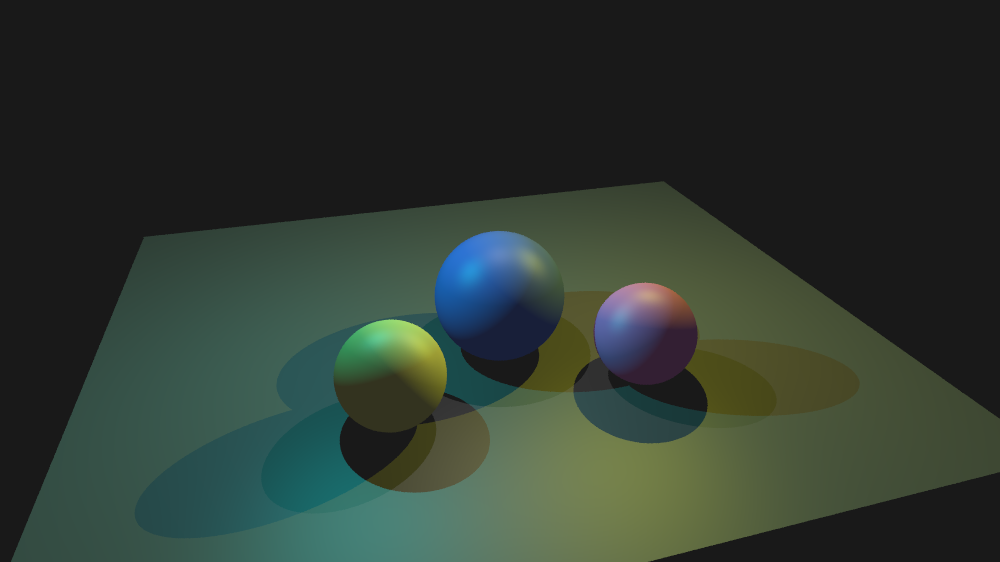
\includegraphics[width=.3\textwidth]{camera3}\quad
		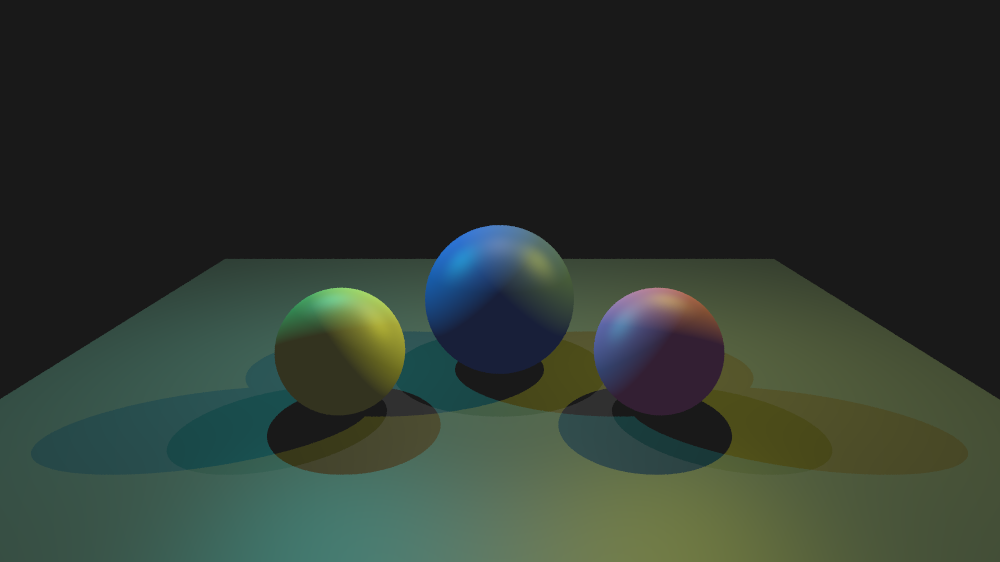
\includegraphics[width=.3\textwidth]{camera1}\quad
		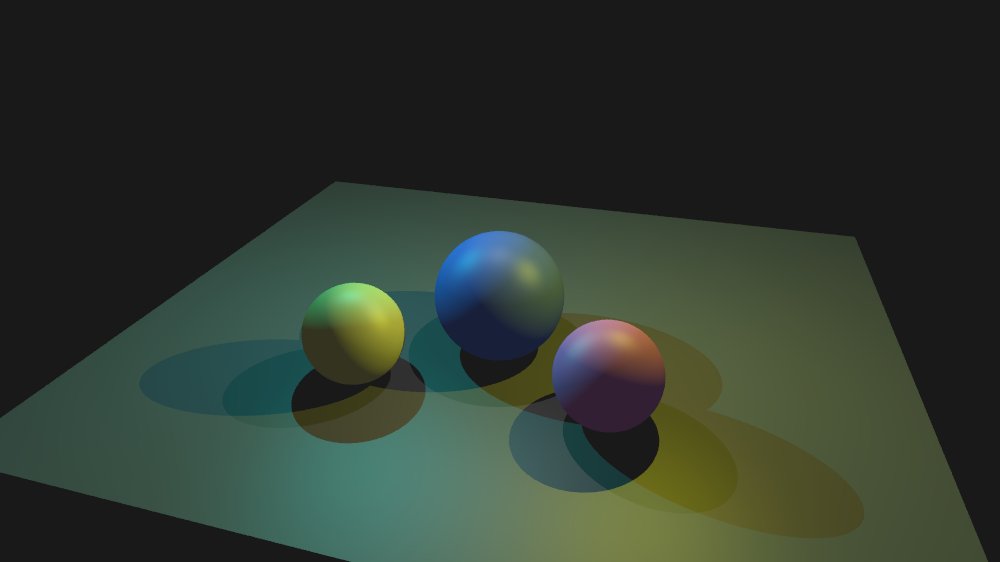
\includegraphics[width=.3\textwidth]{camera2}\quad
		\caption{Three images rendered using the same scene placing camera at different positions. Three point lights of different colors were used to illuminate the scene.}
	\end{figure}
	
	\section{Axis Aligned Bounding Box (Ray-AABB intersection)}

	So far, we have been using the ray-intersection methods we have implemented to check whether a ray hits an object. This means that for every ray that shoots from the camera, we are evaluating our spheres and triangles in our scene by going through their respective ray-intersection methods which can be quite expensive. It would be useful if we could wrap the objects in our scene with a simpler and less expensive ray-intersection method and when we are sure that the method returns true, we can then use the respective ray-intersection method for the actual object (sphere or triangle).
	\begin{figure}[H]
		\centering
		\captionsetup{justification=centering}
		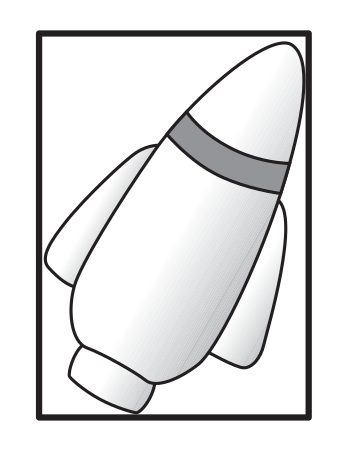
\includegraphics[width=.2\textwidth]{aabb}\quad
		\caption{An axis-aligned bounding box (AABB) enclosing another object \protect\cite{ericson2004real}.}
	\end{figure}
 	\noindent
	This also speeds up the rendering process. It is quite obvious that if a ray does not return true for the less expensive intersection method, we can return from our hit function altogether, without even going through the expensive intersection method for the respective object. One way to achieve this is by using an \textbf{axis-aligned bounding box}. An axis-aligned bounding box completely encloses another object as illustrated in figure 34. It is called axis-aligned because it's axes are parallel to world coordinate axes. There are many methods introduced for ray-AABB intersections but the most dominant method is the \textbf{slabs test} \cite{kay1986ray}.
	\noindent
	A box requires two min and max positions which are the two opposite corners of the box. In 2D, it is represented by two slabs, an $x$-slab and a $y$-slab as shown in figure 35.
	\begin{figure}[H]
		\centering
		\captionsetup{justification=centering}
		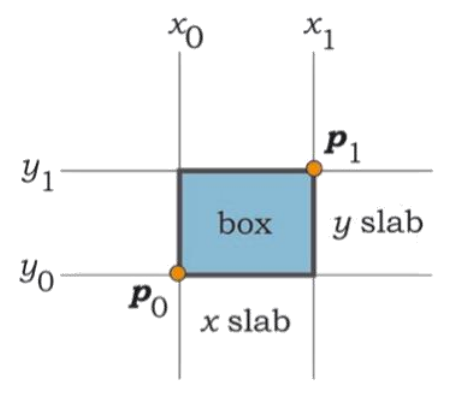
\includegraphics[width=.35\textwidth]{aabb1}\quad
		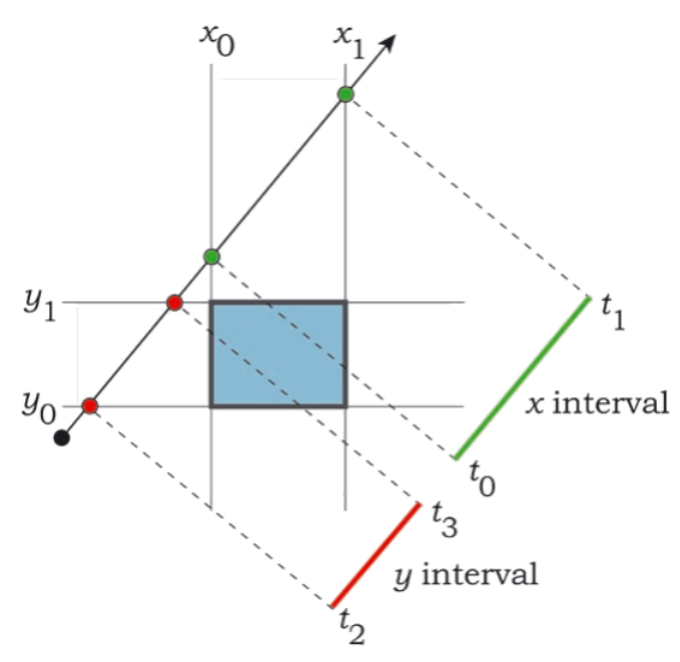
\includegraphics[width=.35\textwidth]{aabb2}\quad
		\caption{Left: A 2D axis-aligned box defined by two slabs. Right: A ray misses the box with non-overlapping $x$ and $y$ intervals \protect\cite{suffern2016ray}.}
	\end{figure}
	\noindent
	For 3D, we would have 3 slabs respectively. In the above figure, $\boldsymbol{p}_{0}$ and $\boldsymbol{p}_{1}$ are the min and max values. Figure 35 (Right) illustrates an example when a ray misses the box. The black arrow indicates the ray and the green dots indicate where the ray passes through the $x$-slab and the red dots indicate where the ray passes through the $y$-slab. The green and red dots create intervals on the ray. These are the intervals when the ray entered and exited the respective slabs. The ray intersects the box if these two intervals overlap which is clearly not the case above. Figure 36 illustrates some cases when a ray intersects the box and it can be seen that the two intervals also overlap.
	\begin{figure}[H]
		\centering
		\captionsetup{justification=centering}
		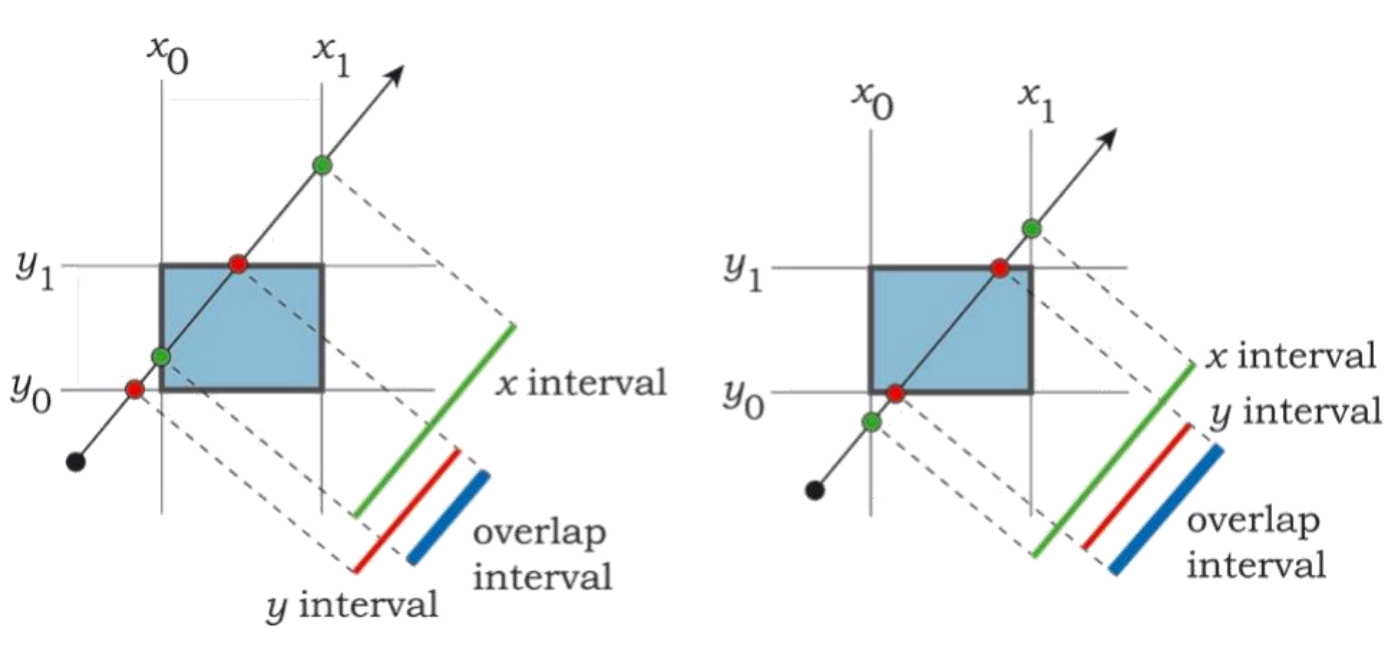
\includegraphics[width=.7\textwidth]{aabb3}\quad
		\caption{Cases where a ray intersects the box \protect\cite{suffern2016ray}.}
	\end{figure}
	\noindent
	For a sphere, the min and max positions are given by:
	\begin{equation}
		\boldsymbol{min}_{aabb} = \boldsymbol{c} - r
	\end{equation}
	\begin{equation}
	\boldsymbol{max}_{aabb} = \boldsymbol{c} + r
	\end{equation}
	where $\boldsymbol{c}$ is the center of the sphere while $r$ is the radius. So radius $r$ is subtracted from each $x$, $y$ and $z$ coordinate of the center $\boldsymbol{c}$ to get $\boldsymbol{min}_{aabb}$ while the radius is added to get $\boldsymbol{max}_{aabb}$. For a triangle, $\boldsymbol{min}_{aabb}$ is the vertex with the minimum value of the $x$, $y$ and $z$ coordinate among all vertices and $\boldsymbol{max}_{aabb}$ is the one with the maximum value. For a mesh, this needs to be checked for all triangles in the mesh and the vertex with the minimum and maximum value is chosen.
	
	\subsection{Analysis of AABB}
	
	Now that we have an AABB implementation we can analyze the difference it makes when using AABBs as a first intersection test to encapsulate meshes in our scenes. When a mesh is loaded in the ray tracer, we will compute its min and max vertices as discussed in the previous section and create an axis-aligned bounding box for it. For every ray that goes into the scene from the camera's origin, if the ray doesn't hit the AABB of the mesh, it also would not hit the mesh itself and so we return from our hit function without doing any expensive computation (ray-triangle intersections). We will use three different scenes for this purpose and evaluate them by first rendering the scene without AABBs and then afterwards rendering the same scene using AABBs. Each of the three scenes were using 5x anti-aliasing, has a plane made up of two triangles with three point lights illuminating the scene:
	\begin{enumerate}
		\item The first scene uses a cube as a mesh made up of 12 triangles.
		\item The second scene uses the stanford bunny \cite{stanfordbunny} as a mesh made up of 4, 968 triangles.
		\item The third scene uses the utah teapot \cite{utahteapot} as a mesh made up of 6, 320 triangles.
	\end{enumerate}
	We will calculate the number of \textbf{ray-mesh intersection} tests which is the number of times it is checked if a ray hits the mesh. We will also be calculating the number of \textbf{ray-triangle intersection} tests which is the number of times it is checked if a ray hits any of the triangles in the mesh. The counter for ray-triangle intersection tests does not take into account the checks for the two triangles that make up the plane as we are not using AABBs to enclose individual triangles. Note that the render times might vary on the machine used to render. These were the results I got on my machine.
	\subsubsection{Scene 1 - Cube}
	\begin{figure}[H]
		\centering
		\captionsetup{justification=centering}
		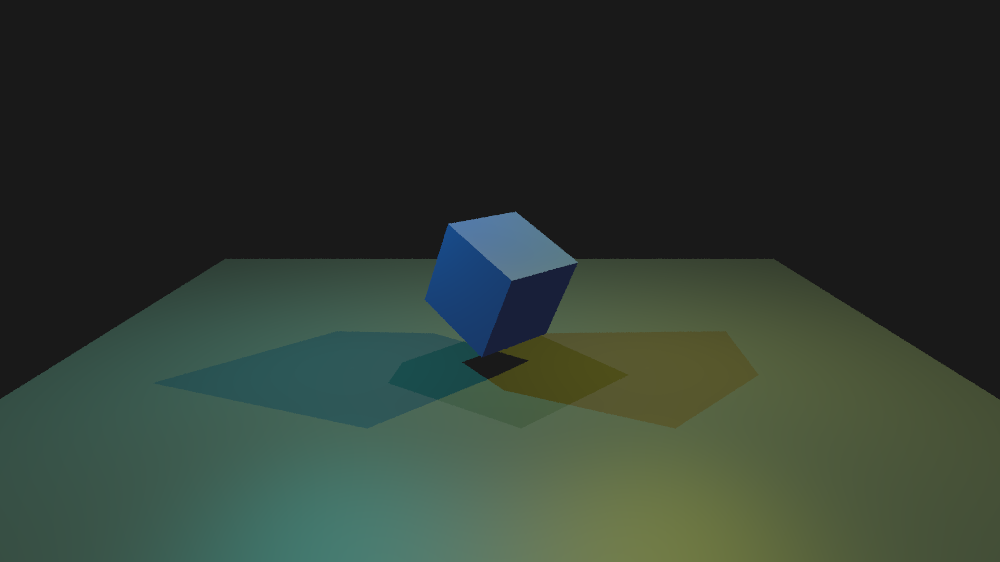
\includegraphics[width=.5\textwidth]{cubescene}\quad
		\caption{Image rendered of a slightly rotated cube.}
	\end{figure}
	
	\begin{table}[h]
		\centering
		\begin{tabular}{ |p{3cm}||p{3cm}|p{3cm}|p{3cm}|  }
			\hline
			\multicolumn{4}{|c|}{Scene 1 - Cube} \\
			\hline
			Type   &   Ray-mesh intersection tests  & Ray-triangle intersection tests &   Time taken to render\\
			\hline
			Without AABB   & 6, 945, 413    &80, 712, 814&   11.16 seconds\\
			With AABB&   1, 186, 019  &11, 600, 086   &      4.98 seconds\\
			\hline
		\end{tabular}
	\end{table}

	\subsubsection{Scene 2 - Stanford Bunny}
	\begin{figure}[H]
		\centering
		\captionsetup{justification=centering}
		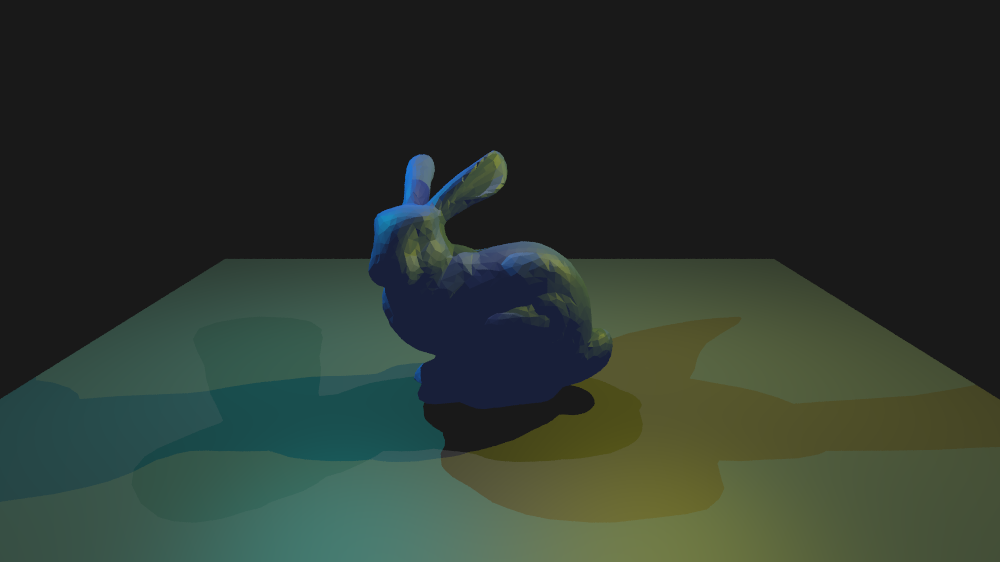
\includegraphics[width=.5\textwidth]{bunnyscene}\quad
		\caption{Image rendered of a stanford bunny.}
	\end{figure}
	
	\begin{table}[h]
		\centering
		\begin{tabular}{ |p{3cm}||p{3cm}|p{3cm}|p{3cm}|  }
			\hline
			\multicolumn{4}{|c|}{Scene 2 - Stanford Bunny} \\
			\hline
			Type   &   Ray-mesh intersection tests  & Ray-triangle intersection tests &   Time taken to render\\
			\hline
			Without AABB   & 7, 017, 974 & 30, 753, 145, 292&   3, 665.91 seconds\\
			With AABB&   3, 280, 692 & 12, 186, 328, 316  &       1, 432.76 seconds\\
			\hline
		\end{tabular}
	\end{table}

	\subsubsection{Scene 3 - Utah Teapot}
	\begin{figure}[H]
		\centering
		\captionsetup{justification=centering}
		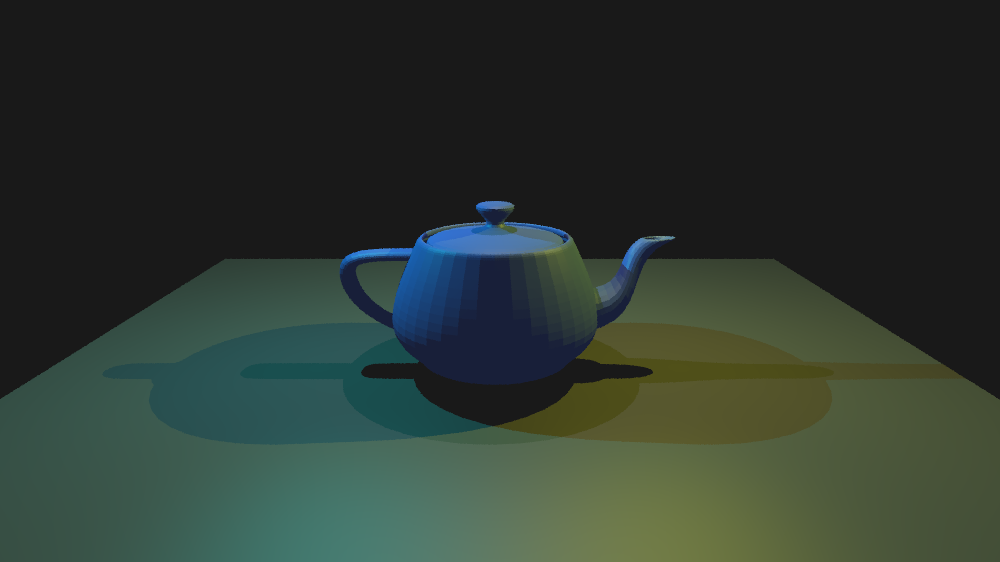
\includegraphics[width=.5\textwidth]{teapotscene}\quad
		\caption{Image rendered of a utah teapot.}
	\end{figure}
	
	\begin{table}[h]
		\centering
		\begin{tabular}{ |p{3cm}||p{3cm}|p{3cm}|p{3cm}|  }
			\hline
			\multicolumn{4}{|c|}{Scene 3 - Utah Teapot} \\
			\hline
			Type   &   Ray-mesh intersection tests  & Ray-triangle intersection tests &   Time taken to render\\
			\hline
			Without AABB   & 6, 987, 782   &40, 894, 443, 281&   3, 817.24 seconds\\
			With AABB&   3, 367, 474 & 18, 014, 096, 721   &       1, 623.18 seconds\\
			\hline
		\end{tabular}
	\end{table}

	\noindent
	It is quite obvious that using AABBs greatly reduces the time it takes to render an image. For the scenes tested, it can be seen that the time was halved from when the scenes were rendered without using AABBs. The intersection tests were also greatly reduced when using AABBs.
	
	\section{Area lights}
	This section is inspired by the online chapter on \textbf{Area Lights} from the book \textbf{The Ray Tracer Challenge} \cite{TRTChallenge}.
	If you observe closely for the images rendered so far, it would be clear that the shadows generated using point lights are hard shadows with sharp edges. 
	\begin{figure}[H]
		\centering
		\captionsetup{justification=centering}
		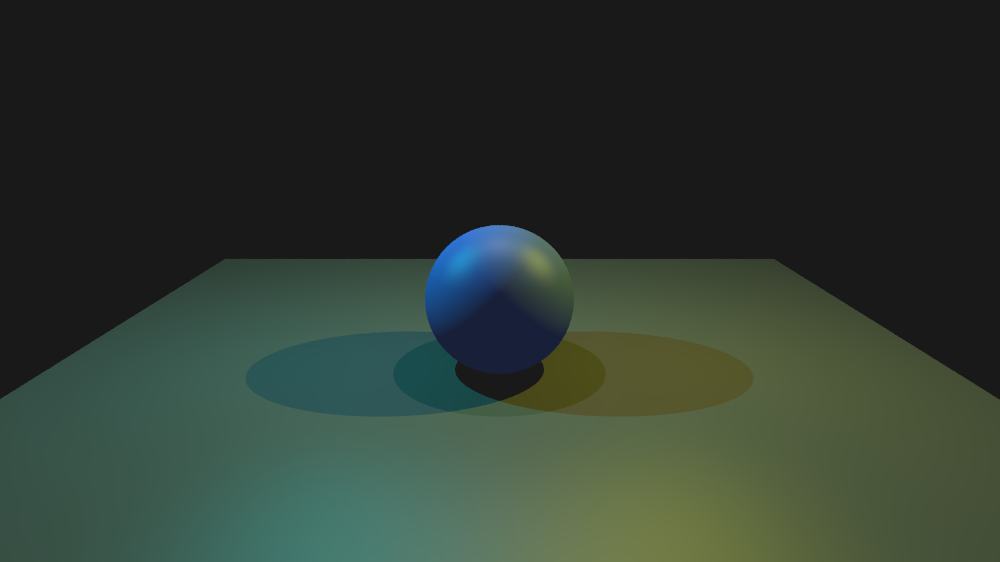
\includegraphics[width=.4\textwidth]{point_light_hard_shadows}\quad
		\caption{Image rendered using three different point lights illuminating the scene. Note the hard shadows created by point lights.}
	\end{figure}
	\noindent
	A sphere would give an exact shadow of the shape of a sphere while this is not true when we observe shadows in real life. All light sources in real life such as a light bulb or a tube light have physical dimensions, which means that a point on an object can only be partially visible from these light sources. This partial occlusion, creates a \textbf{penumbra}, which is the part of a shadow where the light source is only partially blocked \cite{penumbra}. This results in more realistic looking shadows known as \textbf{soft shadows}.
	\begin{figure}[H]
		\centering
		\captionsetup{justification=centering}
		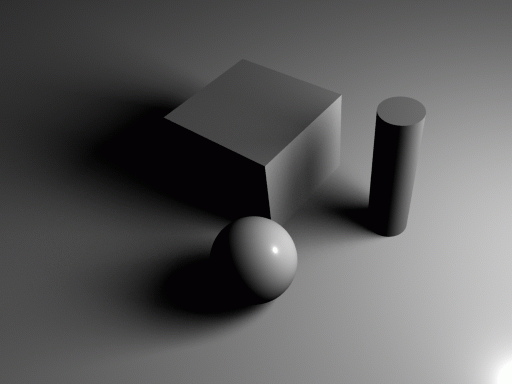
\includegraphics[width=.3\textwidth]{softshadows}\quad
		\caption{Soft shadows \protect\cite{christensen2018renderman}.}
	\end{figure}
	\noindent
	Soft shadows can be achieved using a different type of light source known as \textbf{area light}. Area lights, unlike point lights, are not a single point of light source but can be think of as a bunch of light sources around a given position $\boldsymbol{l}_{p}$. Since we already have a point light implementation, we can use the same by using a number of point lights scattered around a given position. The current setting can be visualized as:
	\begin{figure}[H]
		\centering
		\captionsetup{justification=centering}
		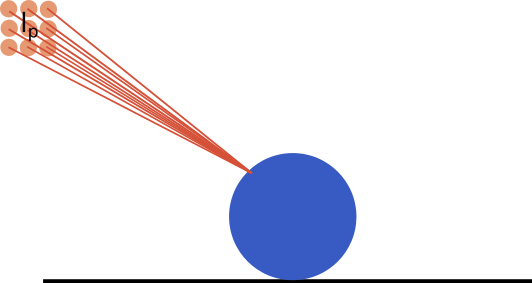
\includegraphics[width=.4\textwidth]{arealight1}\quad
		\caption{Point lights arranged in a 3x3 grid around a position $\boldsymbol{l}_{p}$.}
	\end{figure}
	 \noindent
	 Note that the above figure is only a 2D representation of how the lights are scattered while we're working in 3D. Let's try rendering the above setting.
	 \begin{figure}[H]
	 	\centering
	 	\captionsetup{justification=centering}
	 	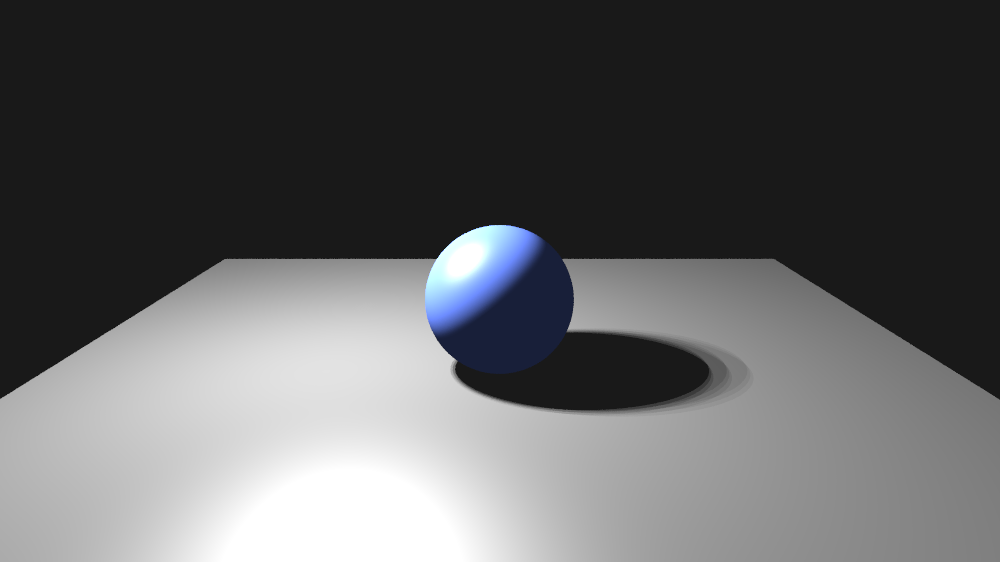
\includegraphics[width=.4\textwidth]{arealight2}\quad
	 	\caption{Image rendered using the setting discussed above. 9 (3x3) point lights of white color were used to illuminate the scene.}
	 \end{figure}
 	\noindent
 	A lot of things went wrong here. First, the sphere looks overexposed to light resulting in an incorrect shading. Second, while the shadows look different, they appear as if a number of shadows were combined on top of each other. We will tackle both of these problems one by one.
 	\\~\\
 	\noindent
 	First, let's look at why the objects in our scene look overexposed to light. Since, we were using point lights, each of them had an intensity value $l_{i}$. The above rendered image had an intensity value of $30$. And since we had 9 point lights scattered around a position $\boldsymbol{l}_{p}$, each of them had an intensity value of $30$ and what we got was a combined effect in our image. What we really want to do is scale that intensity value according to the number of point lights we have in an area light. So, our intensity value should be scaled as:
 	\begin{equation}
 		l_{i} = \frac{l_{i}}{l_{n}}
 	\end{equation}
 	\noindent
 	Where $l_{i}$ is the intensity value of a given point light and $l_{n}$ is the total number of point lights in our scene (9 in our setting above). Let's render the scene again using the scaling we discussed.
 	\begin{figure}[H]
 		\centering
 		\captionsetup{justification=centering}
 		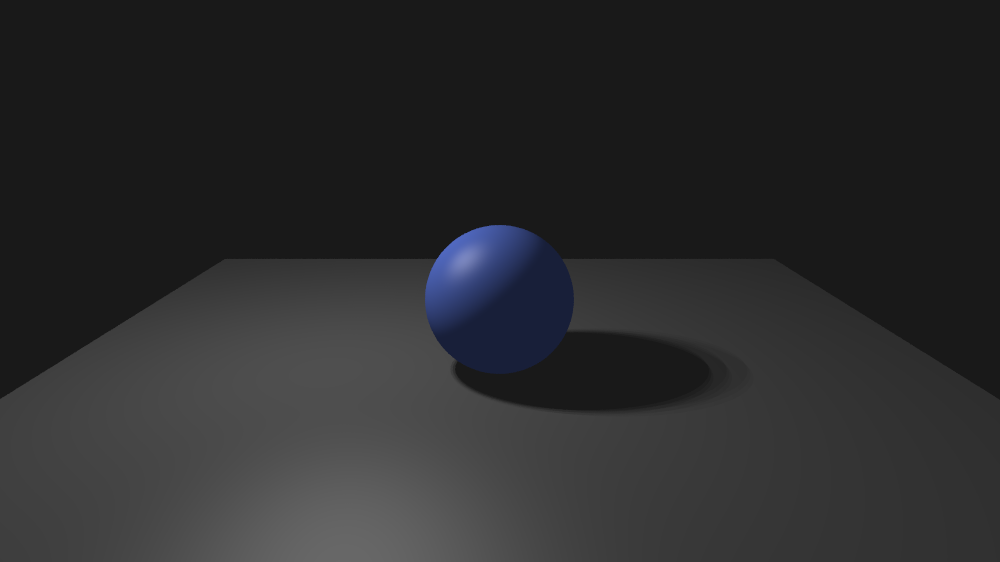
\includegraphics[width=.4\textwidth]{arealight3}\quad
 		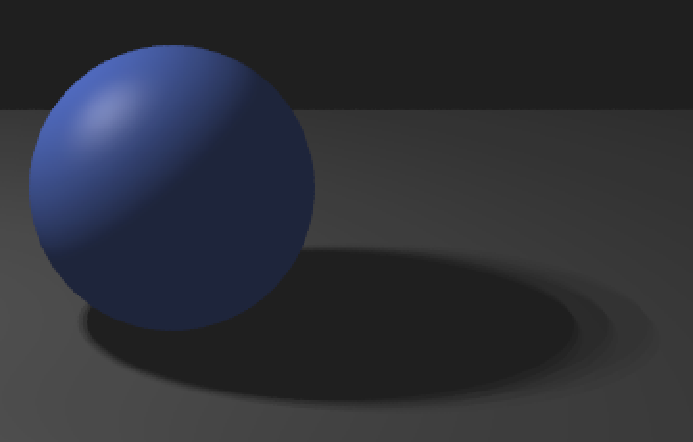
\includegraphics[width=.365\textwidth]{wrongshadows}\quad
 		\caption{Left: Image rendered again with scaled intensity. Right: Incorrect shadows being rendered.}
 	\end{figure}
 	\noindent
 	This looks better but we still need to fix the incorrect shadows. This phenomenon is often called as \textbf{banding} where we get a series of stripes (bands) similar to what is happening with our shadows right now. This is happening in our case because we have point lights equally spaced from one another. What we can do to overcome this issue is, sample the positions of our point lights randomly. 
 	\begin{figure}[H]
 		\centering
 		\captionsetup{justification=centering}
 		\includegraphics[width=.4\textwidth]{arealight4}\quad
 		\caption{Point lights arranged in a 3x3 grid but moved slightly away from their default position.}
 	\end{figure}
 	\noindent
 	More simply, we move our point lights slightly away from their default position, using a radius $r$ that defines how much we want to move our point lights away from their default position. This can be written as:
 	\begin{equation}
 		\boldsymbol{l}_{p} = \boldsymbol{l}_{p} + r * (2 * \eta - 1)
 	\end{equation}
 	\noindent
 	In the equations above, $\eta$ is a random decimal value in the range of $[0, 1)$ and $l_{p}$ is the default position of an individual point light. Rendering an image again after adding random sampling of positions gives us this image:
 	\begin{figure}[H]
 		\centering
 		\captionsetup{justification=centering}
 		\includegraphics[width=.5\textwidth]{arealight5}\quad
 		\caption{Image rendered after adding random sampling of light positions $\boldsymbol{l}_{p}$.}
 	\end{figure}
 	\noindent
 	While, it is not clear in the image above, random sampling also results in noisy images. This is noticeable when we reduce our point lights to a 2x2 grid and increase the light intensity to $60$. One motivation to use a smaller grid is to reduce the time it takes to render our image as now we have a total of 4 point lights instead of 9 (3x3 grid) previously.
 	\begin{figure}[H]
 		\centering
 		\captionsetup{justification=centering}
 		\includegraphics[width=.35\textwidth]{arealight6}\quad
 		\includegraphics[width=.32\textwidth]{noisy}\quad
 		\caption{Image rendered using a 2x2 grid of point lights with a light intensity of $60$.}
 	\end{figure}
 	\noindent
 	Unfortunately there is no perfect solution to this issue. We can increase the grid size which tends to reduce the noise but then the image takes more time to render so it is always a trade off between time and quality. There are many papers that tend to reduce noise or the amount of time it takes to render images when using area lights and soft shadows but we will not be discussing them here. Let us now render the same image we rendered (figure 40) at the start of this section using area lights.
 
	 \begin{figure}[H]
	 	\centering
	 	\captionsetup{justification=centering}
	 	\includegraphics[width=.5\textwidth]{arealight7}\quad
	 	\caption{Image rendered using three different area lights illuminating the scene. Note the soft shadows created by area lights.}
	 \end{figure}
 
 	\section{Final remarks}
 	This lab was a great way to gain practical experience of the concepts we learned in our computer graphics course. I would like to thank \textbf{Prof. Dr.-Ing. Matthias Teschner} again for advising me throughout this lab. As a final remark, I would like to mention that I really enjoyed working on area lights. This includes debugging issues as I was working on them as well as how they were fixed. At the end, the results were worth the effort.

	\bibliographystyle{apacite}
	\bibliography{References}
	
\end{document}